
We evaluate the performance of the proposed methodology for the task of human body pose correspondence estimation, as well as non-rigid alignment ``in-the-wild''. For further experimental results, please refer to the supplementary material. Note that all steps of the proposed pipeline were implemented using the Menpo Project~\cite{menpo14}.

%Results of quantitative and qualitative evaluations are reported.

\begin{figure}[t!]
    \centering
    \includegraphics[width=\columnwidth]{resources/Fig_Variance/final}
    \caption{Example of human pose annotation for left arm among 4 annotators. The large variance highlights the difficulty of obtaining consistent landmarks.}
    \label{fig:variance}
\end{figure}

\begin{figure*}[!t]
    \newcommand{\fh}{0.24\columnwidth}
    \centering
    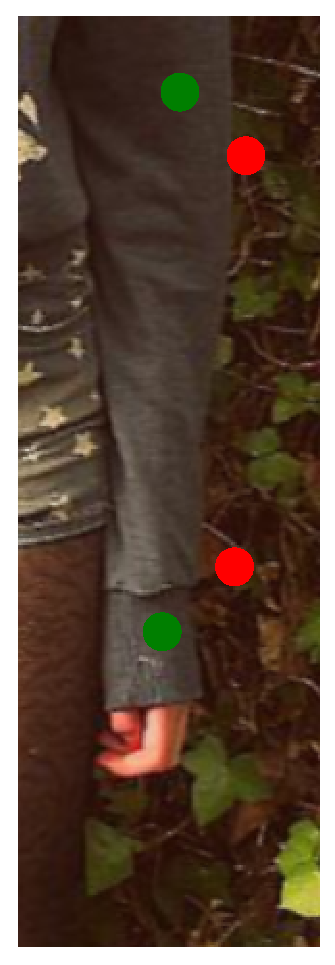
\includegraphics[height=\fh]{resources/Fixing/fix_1}
    \hfill
    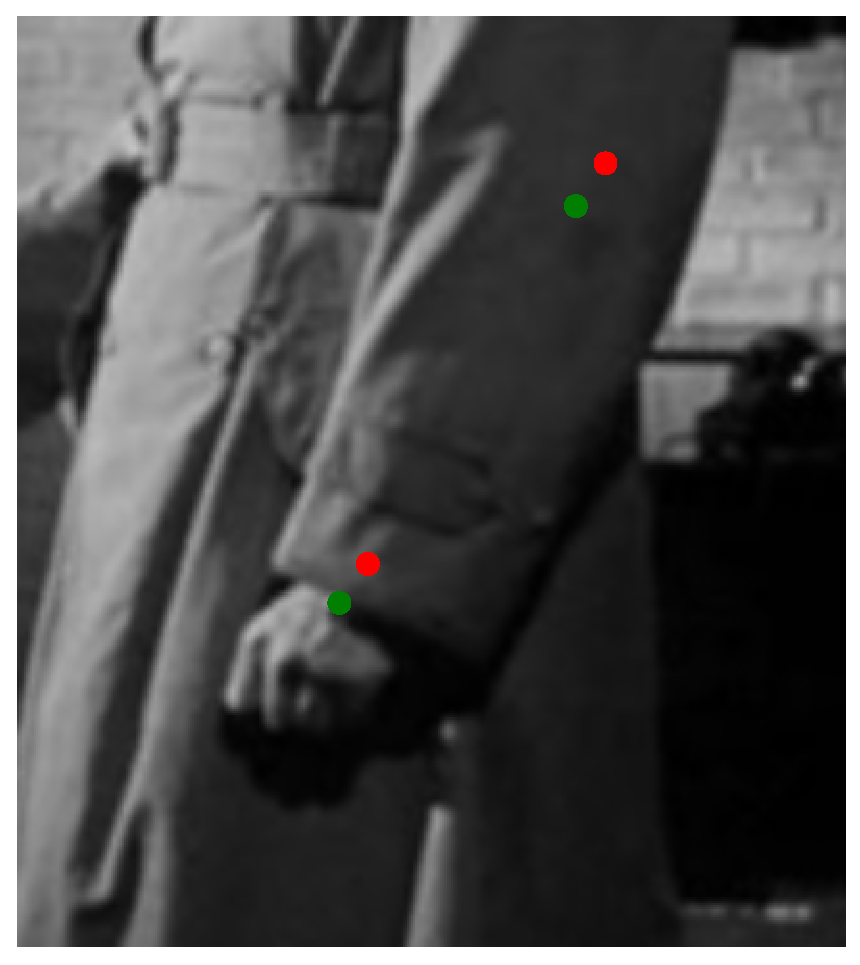
\includegraphics[height=\fh]{resources/Fixing/fix_2}
    \hfill
    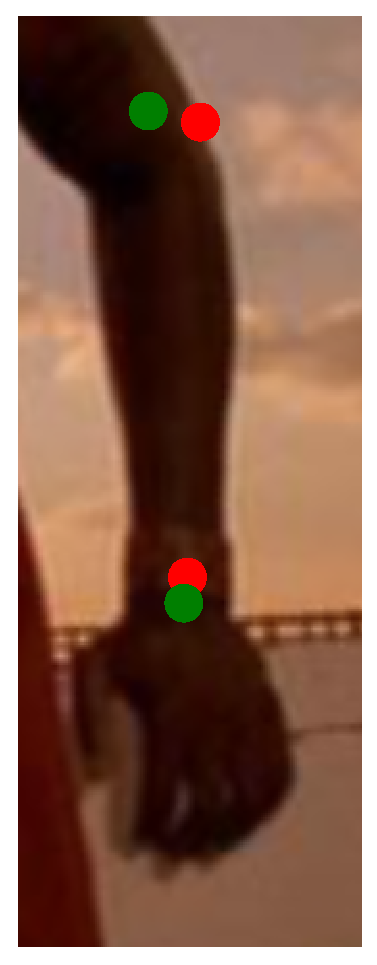
\includegraphics[height=\fh]{resources/Fixing/fix_3}
    \hfill
    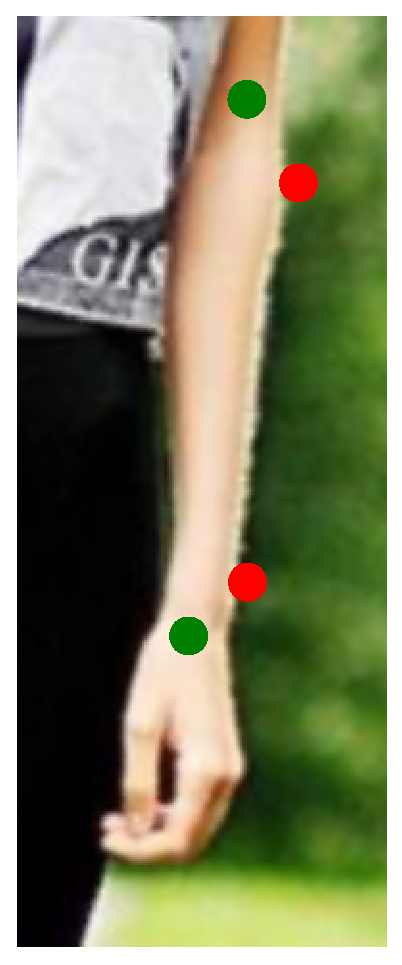
\includegraphics[height=\fh]{resources/Fixing/fix_5}
    \hfill
    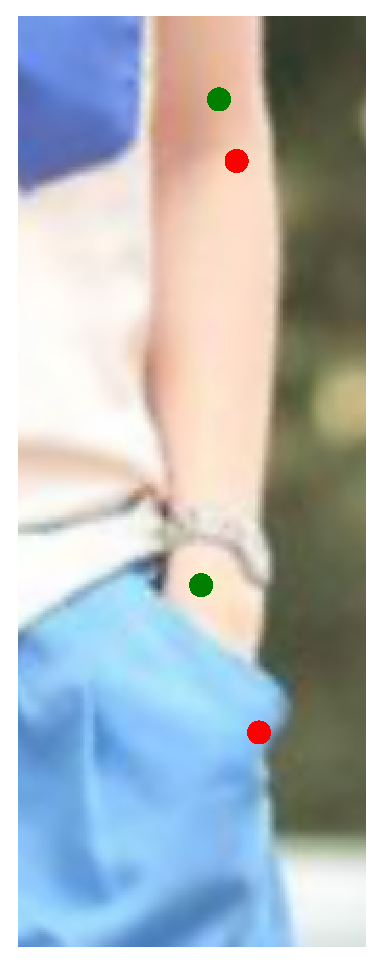
\includegraphics[height=\fh]{resources/Fixing/fix_6}
    \hfill
    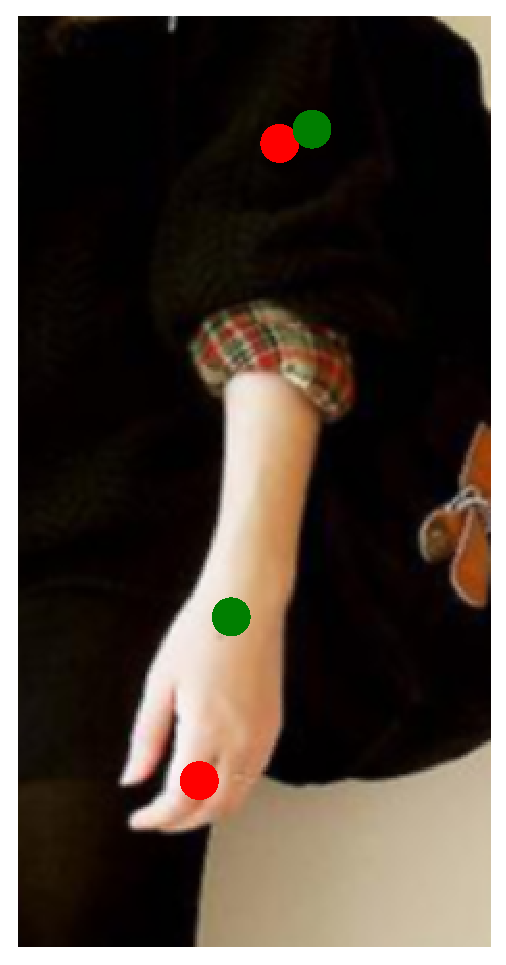
\includegraphics[height=\fh]{resources/Fixing/fix_7}
    \hfill
    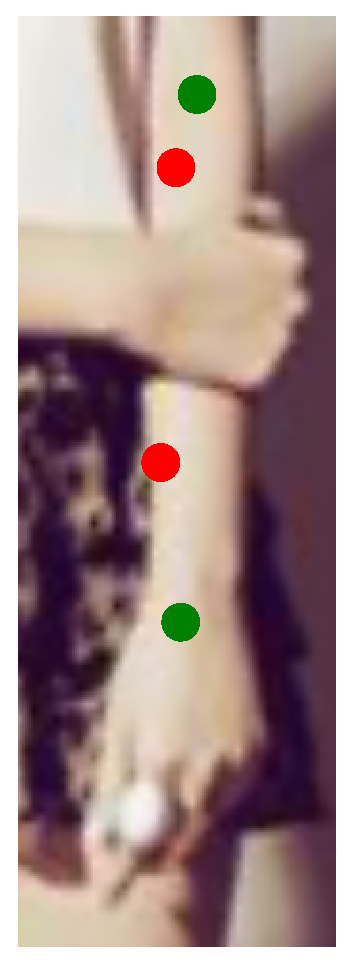
\includegraphics[height=\fh]{resources/Fixing/fix_8}
    \hfill
    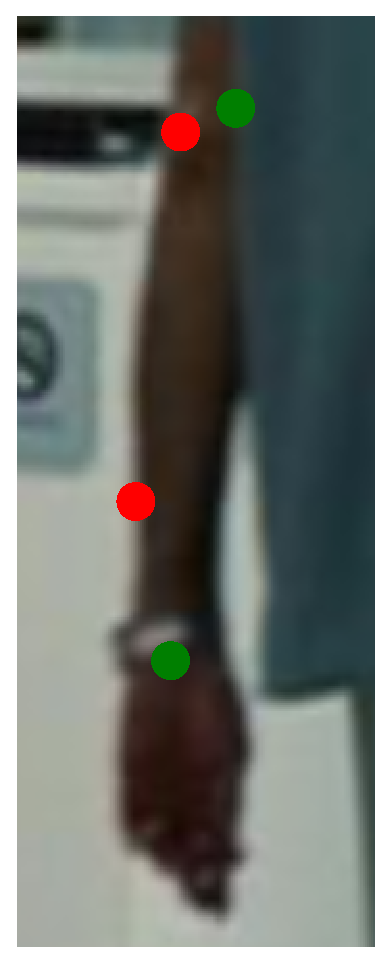
\includegraphics[height=\fh]{resources/Fixing/fix_9}
    \hfill
    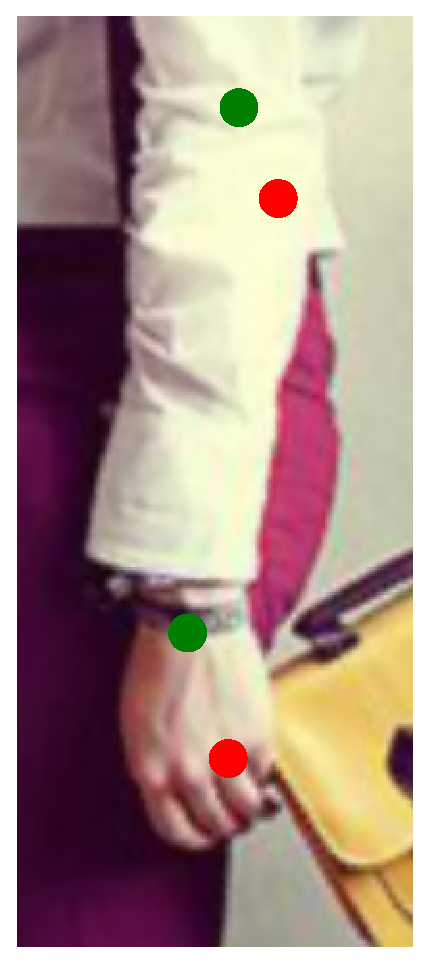
\includegraphics[height=\fh]{resources/Fixing/fix_10}
    \hfill
    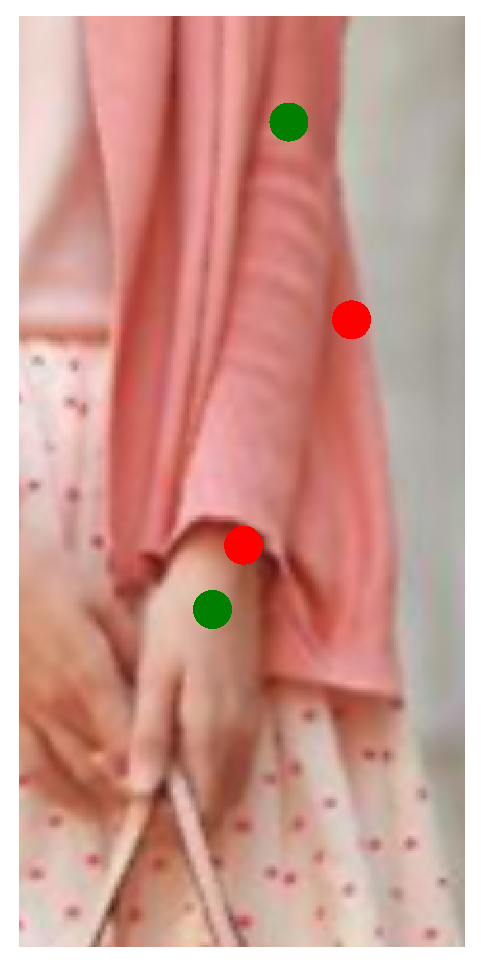
\includegraphics[height=\fh]{resources/Fixing/fix_20}
    \hfill
    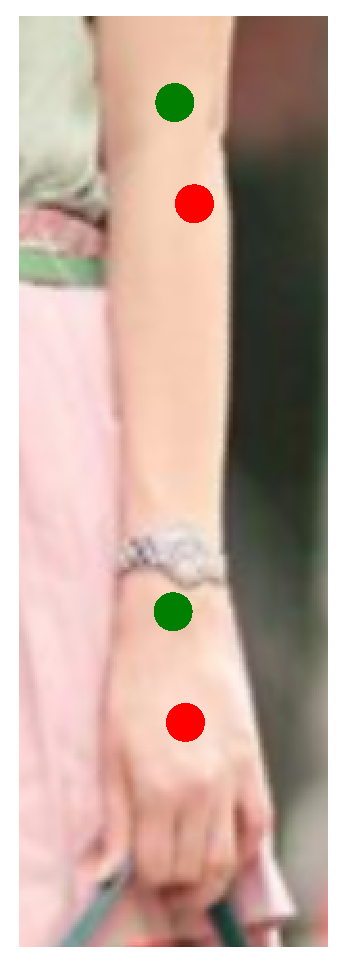
\includegraphics[height=\fh]{resources/Fixing/fix_12}
    \hfill
    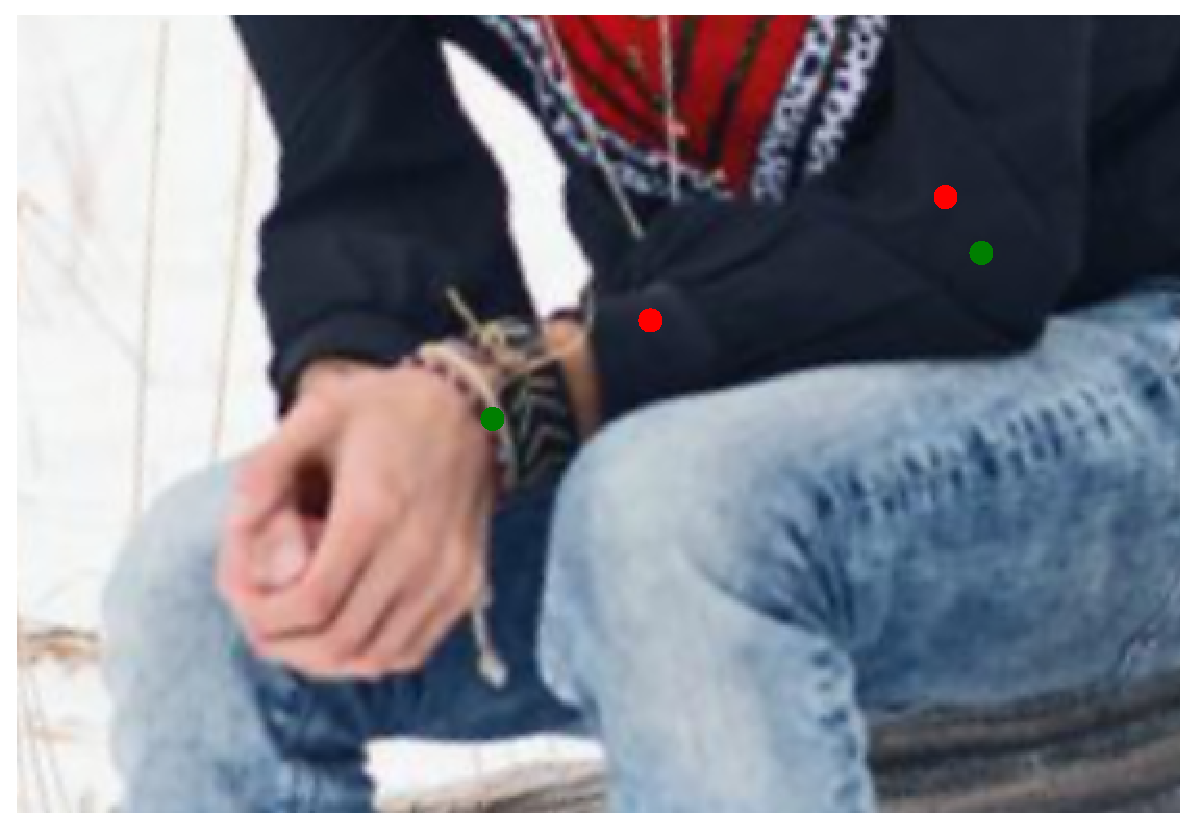
\includegraphics[height=\fh]{resources/Fixing/fix_13}
    \hfill
    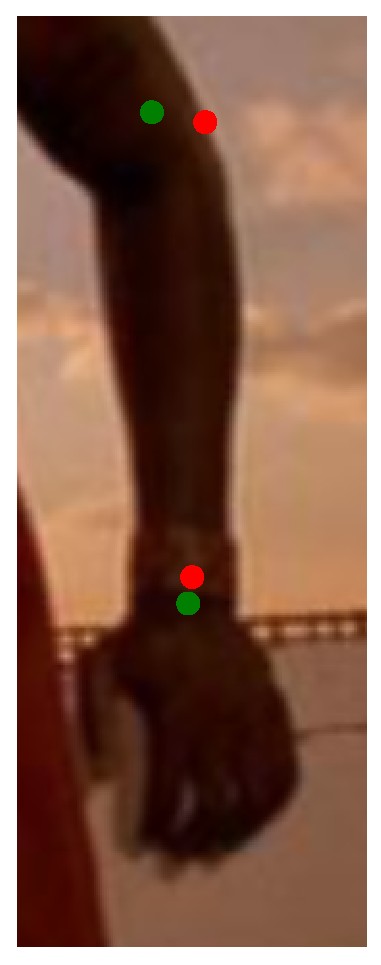
\includegraphics[height=\fh]{resources/Fixing/fix_14}
    \hfill
    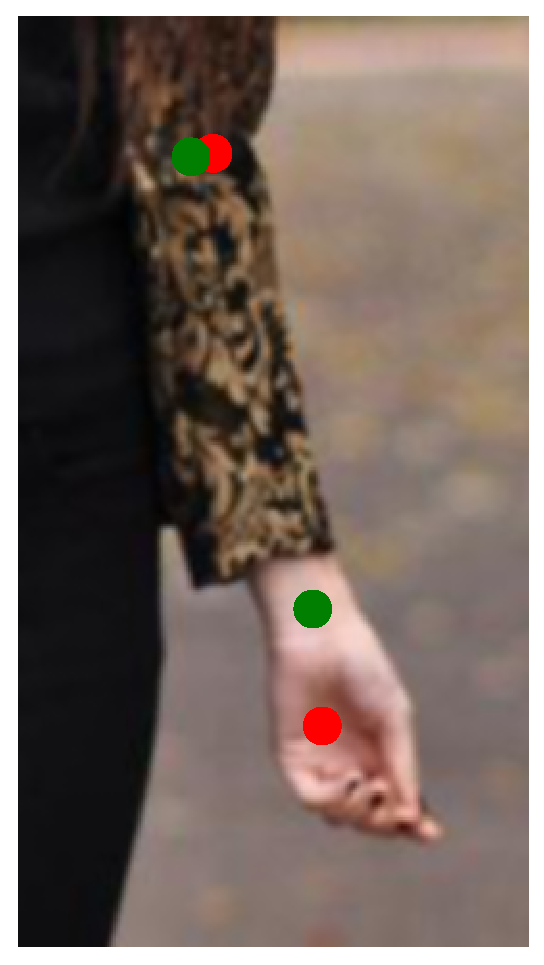
\includegraphics[height=\fh]{resources/Fixing/fix_15}
    \hfill
    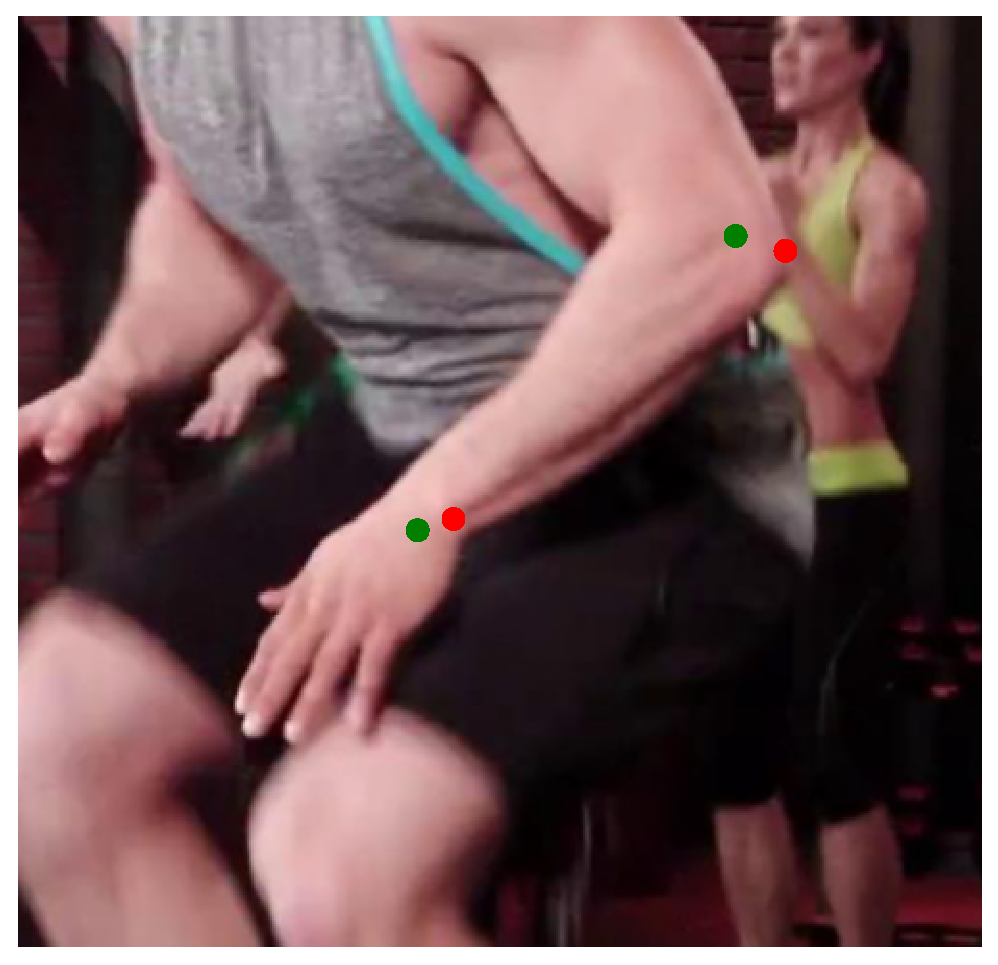
\includegraphics[height=\fh]{resources/Fixing/fix_17}
    \hfill
    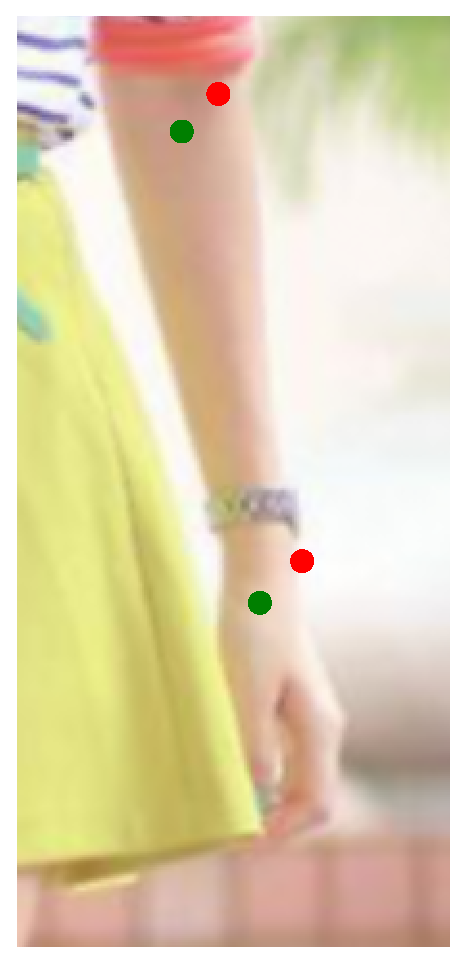
\includegraphics[height=\fh]{resources/Fixing/fix_18}
    \caption{Demonstration of annotation correction using our method for the experiment of Section \ref{exp:qualitative}. \emph{Red} dots refer to officially provided landmarks, and \emph{green} dots are corrected position.}
    \label{fig:qualitative}
\end{figure*}

\begin{figure*}[!t]
    \newcommand{\ofh}{0.24\columnwidth}
    \centering
    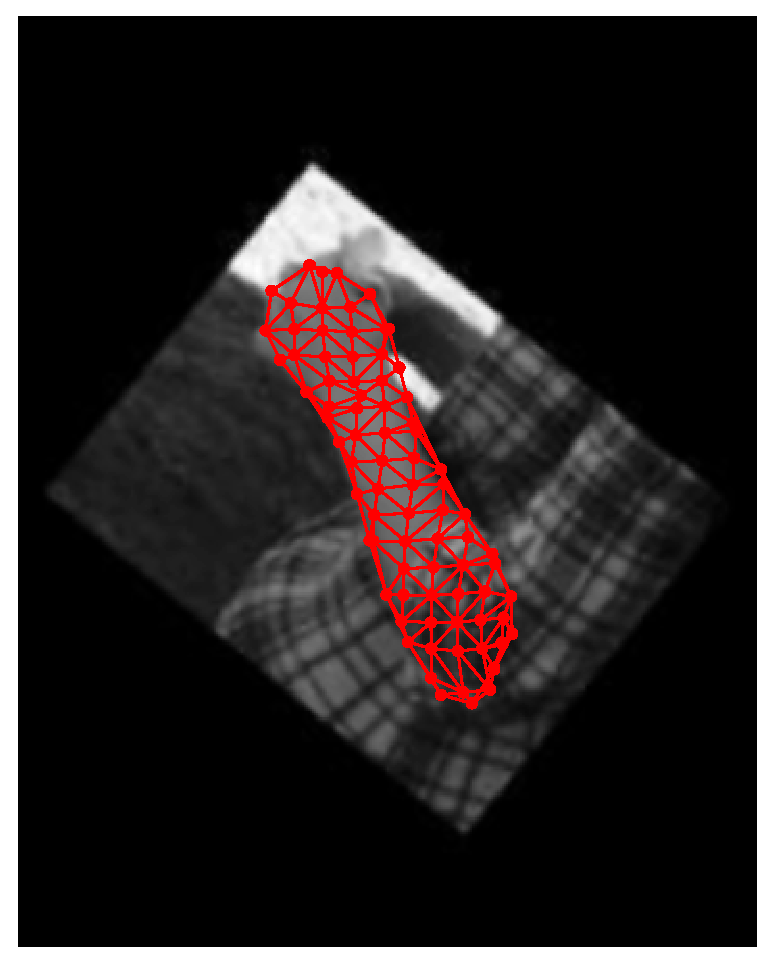
\includegraphics[height=\ofh]{resources/Fittings/20.eps}
    \hfill
    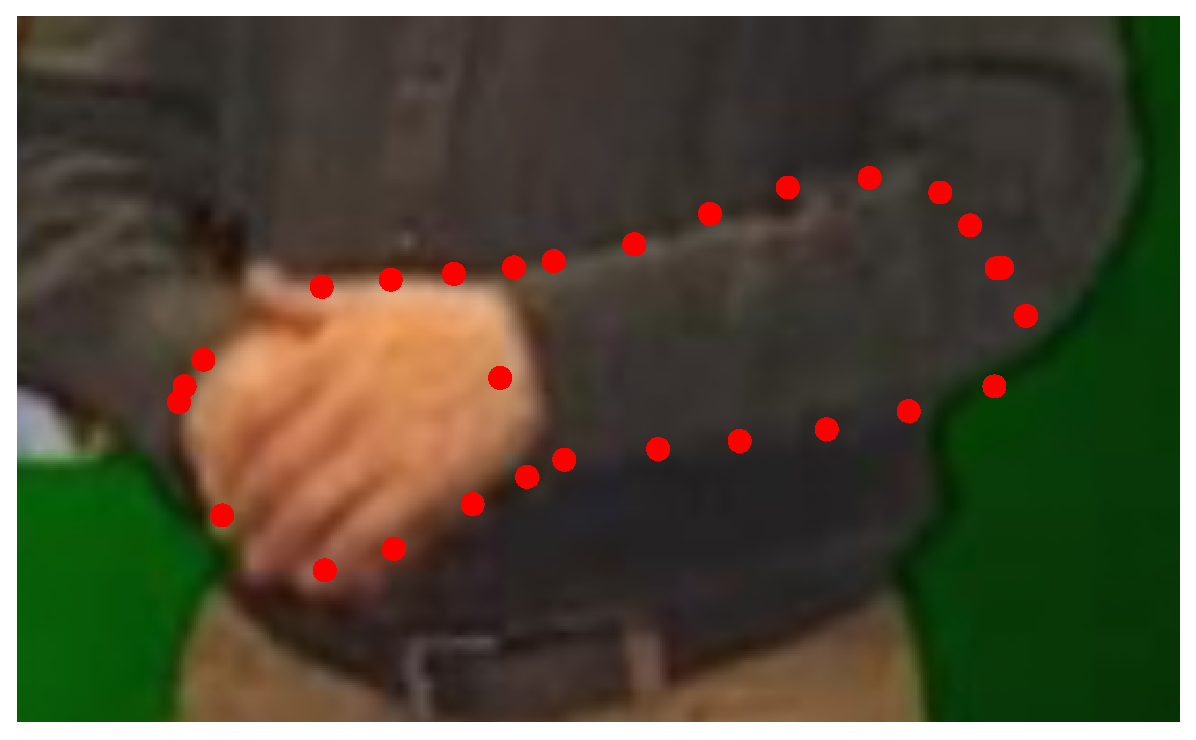
\includegraphics[height=\ofh]{resources/Fittings/3.eps}
    \hfill
    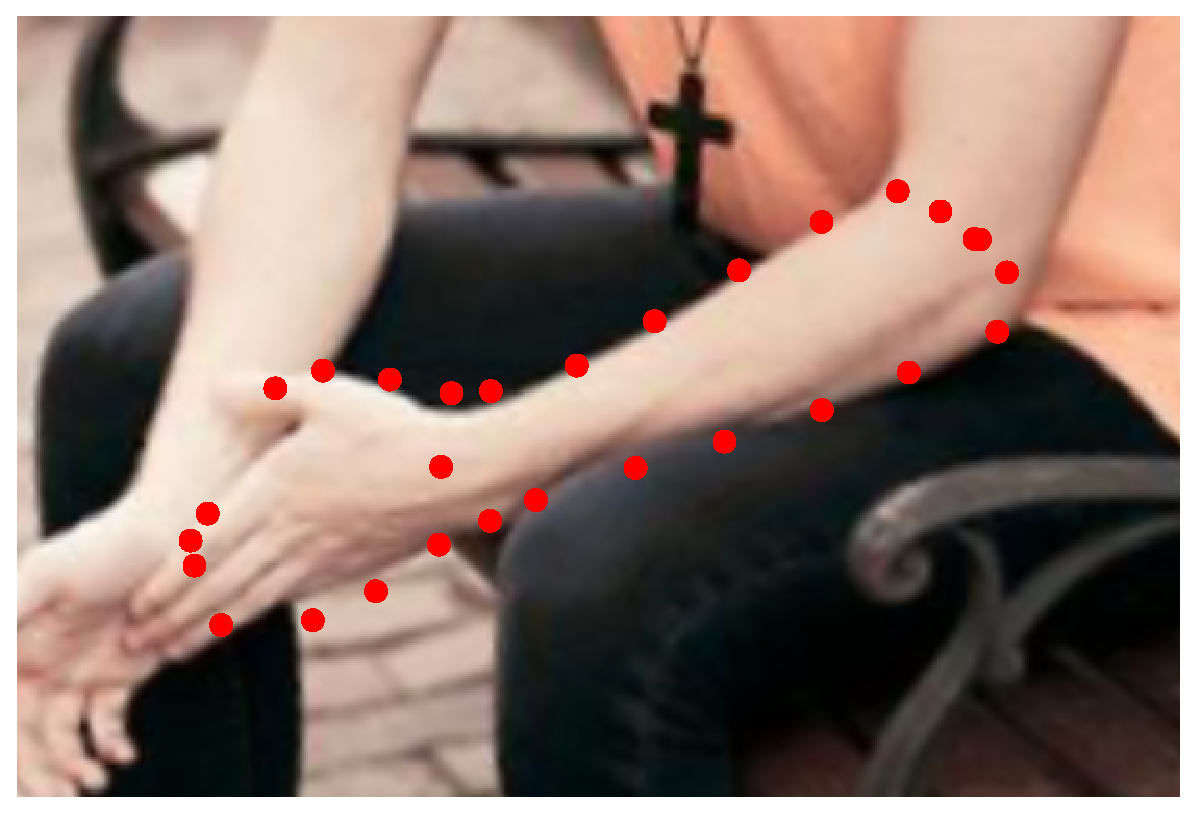
\includegraphics[height=\ofh]{resources/Fittings/19.eps}
    \hfill
    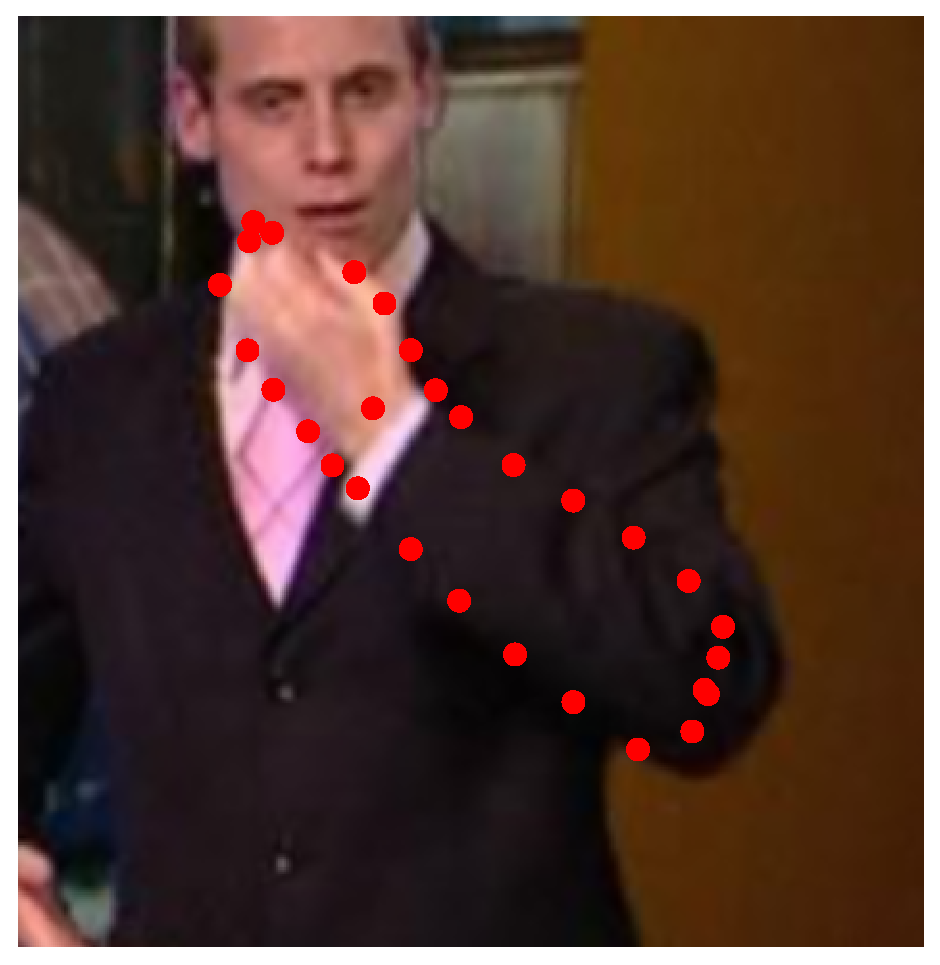
\includegraphics[height=\ofh]{resources/Fittings/4.eps}
    \hfill
    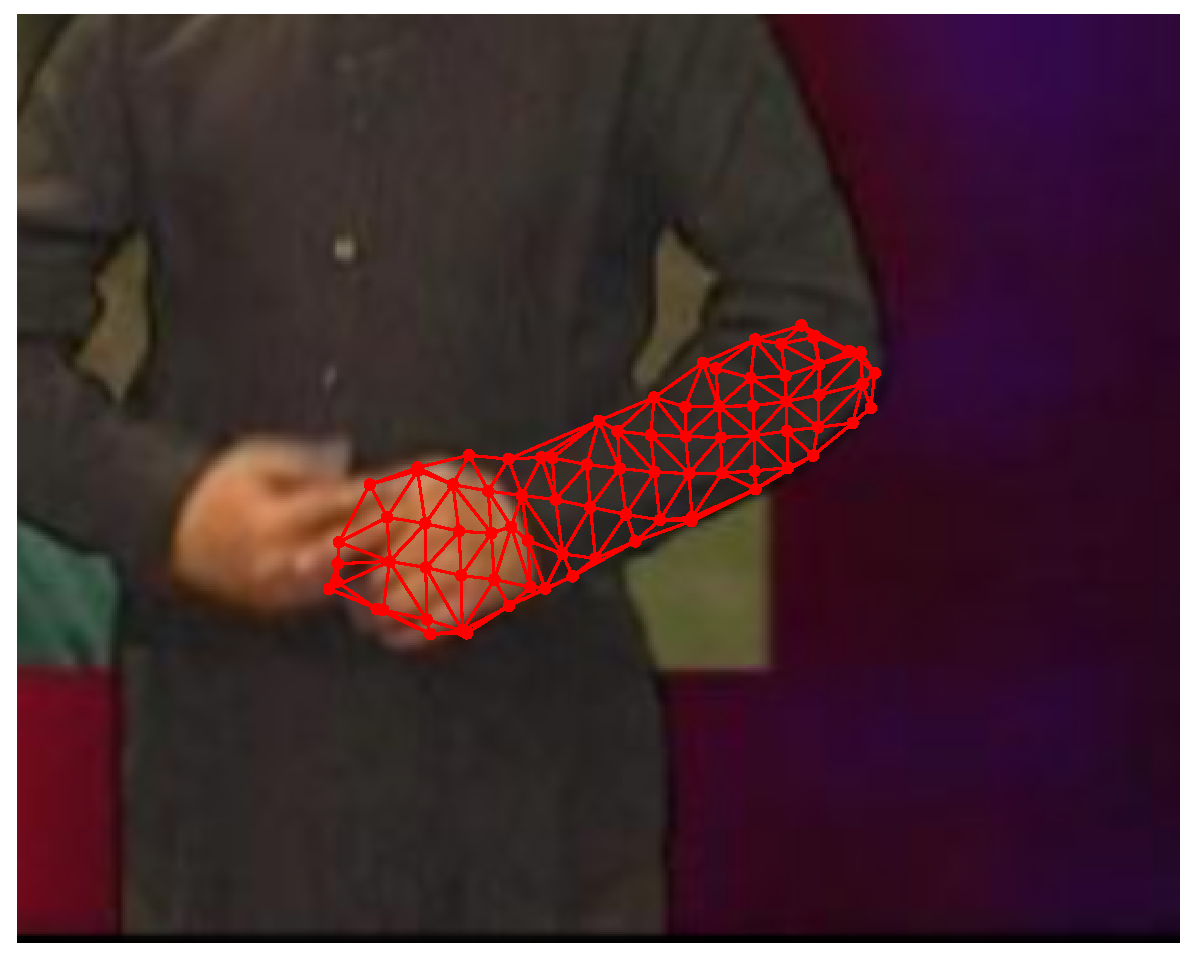
\includegraphics[height=\ofh]{resources/Fittings/6.eps}
    \hfill
    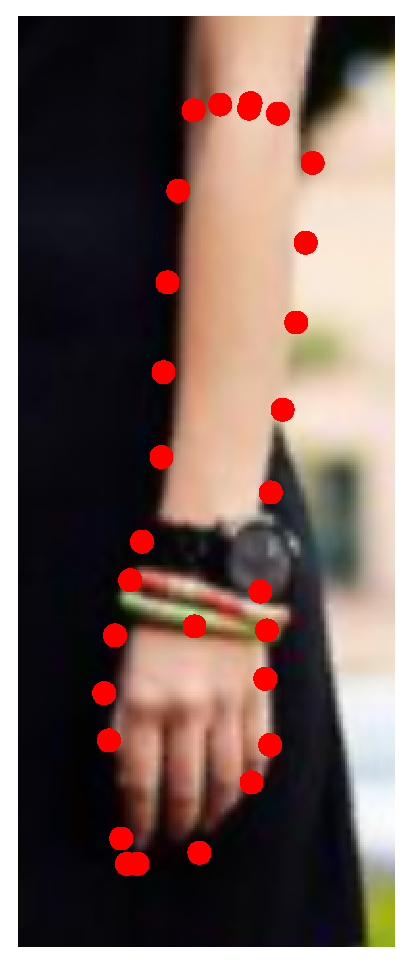
\includegraphics[height=\ofh]{resources/Fittings/15.eps}
    \hfill
    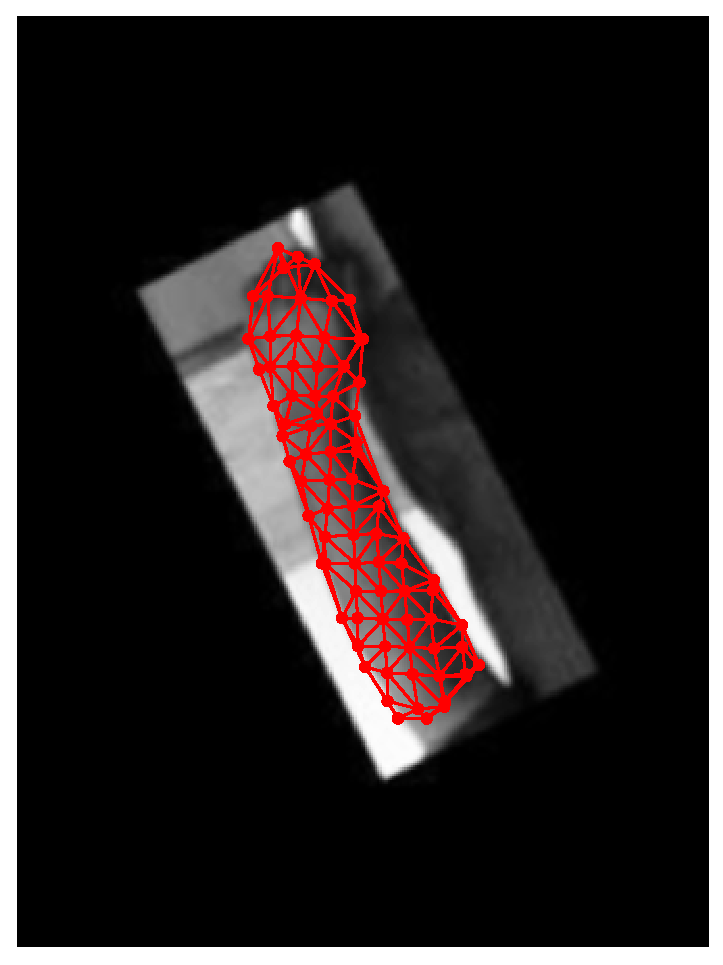
\includegraphics[height=\ofh]{resources/Fittings/7.eps}
    \hfill
    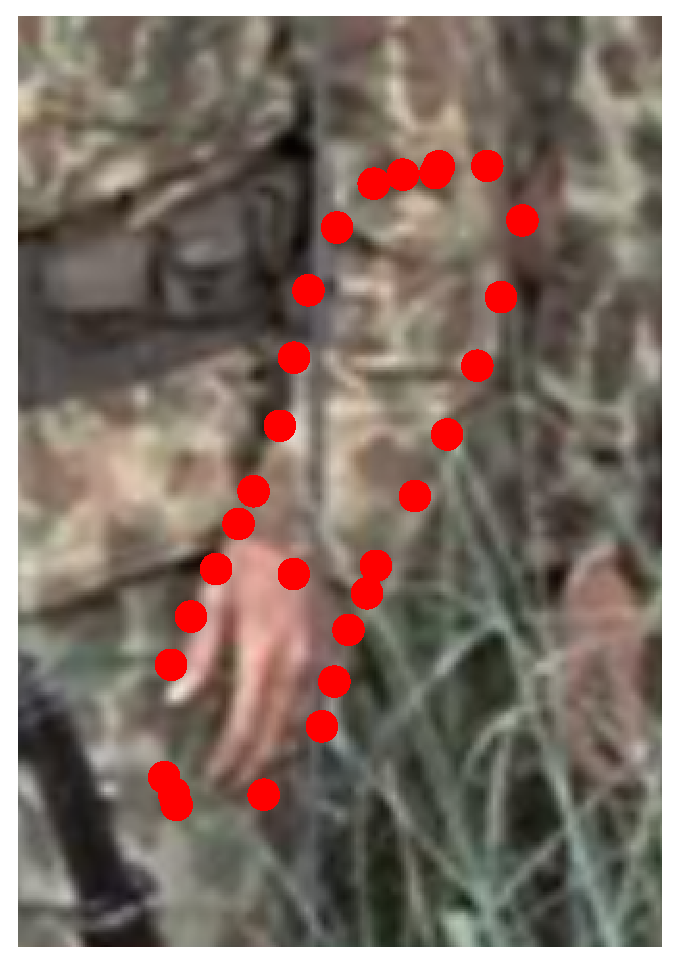
\includegraphics[height=\ofh]{resources/Fittings/8.eps}
    \hfill
    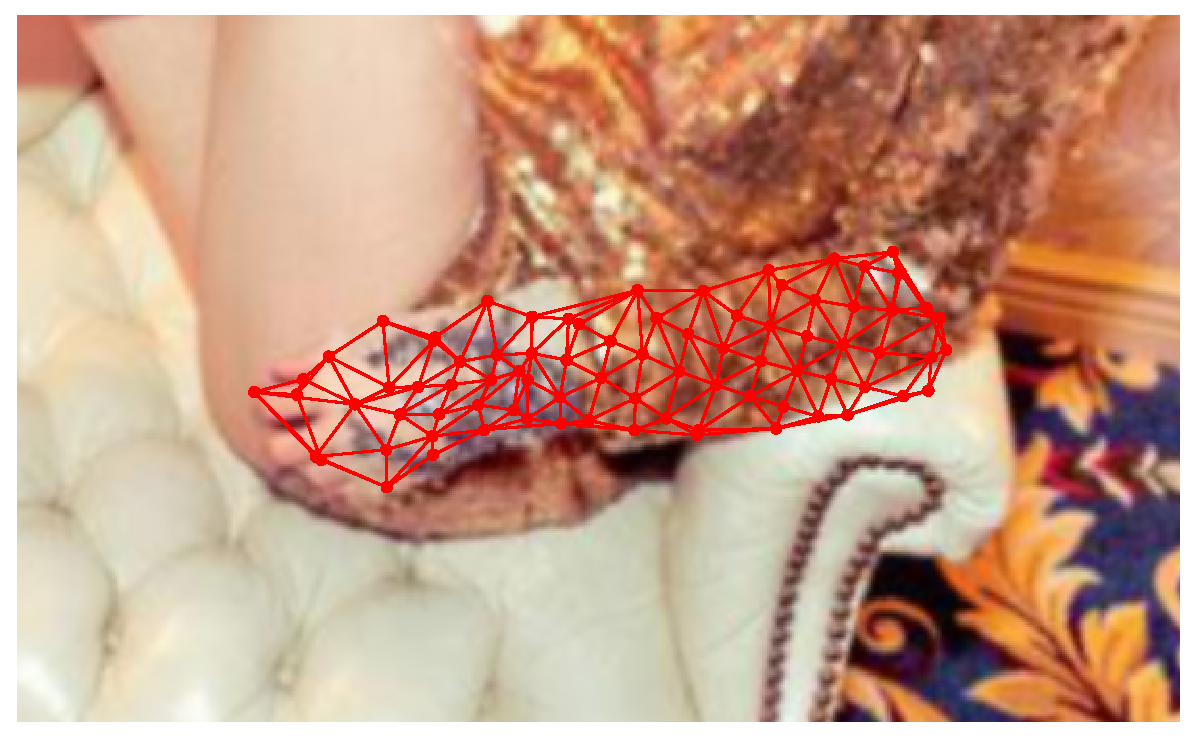
\includegraphics[height=\ofh]{resources/Fittings/13.eps}
    \hfill
    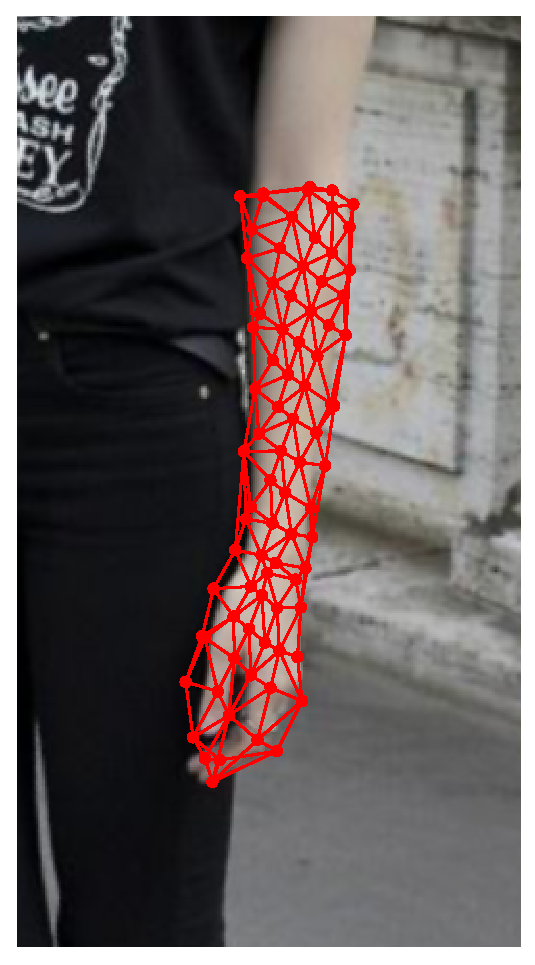
\includegraphics[height=\ofh]{resources/Fittings/17.eps}
    \\
    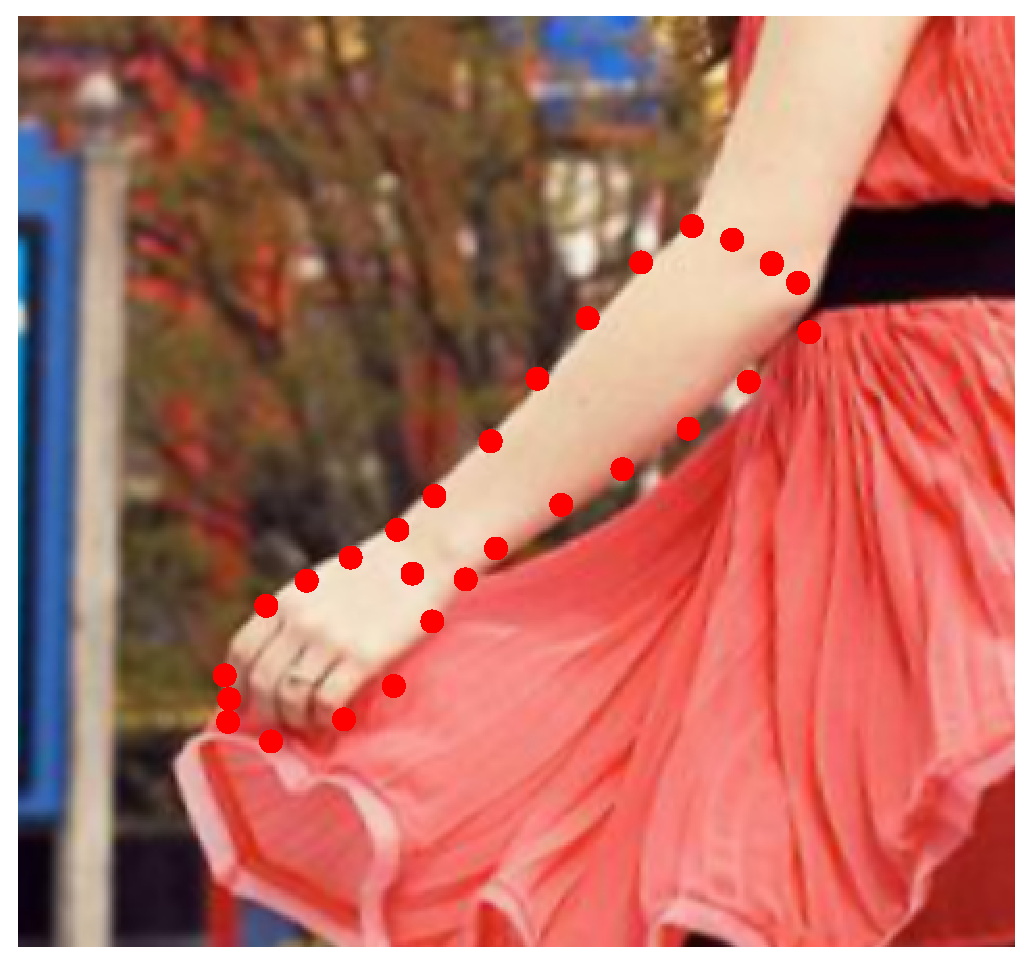
\includegraphics[height=\ofh]{resources/Fittings/21.eps}
    \hfill
    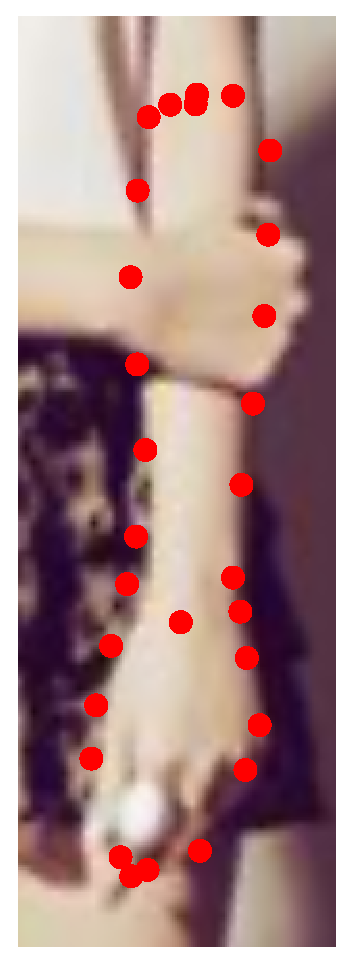
\includegraphics[height=\ofh]{resources/Fittings/23.eps}
    \hfill
    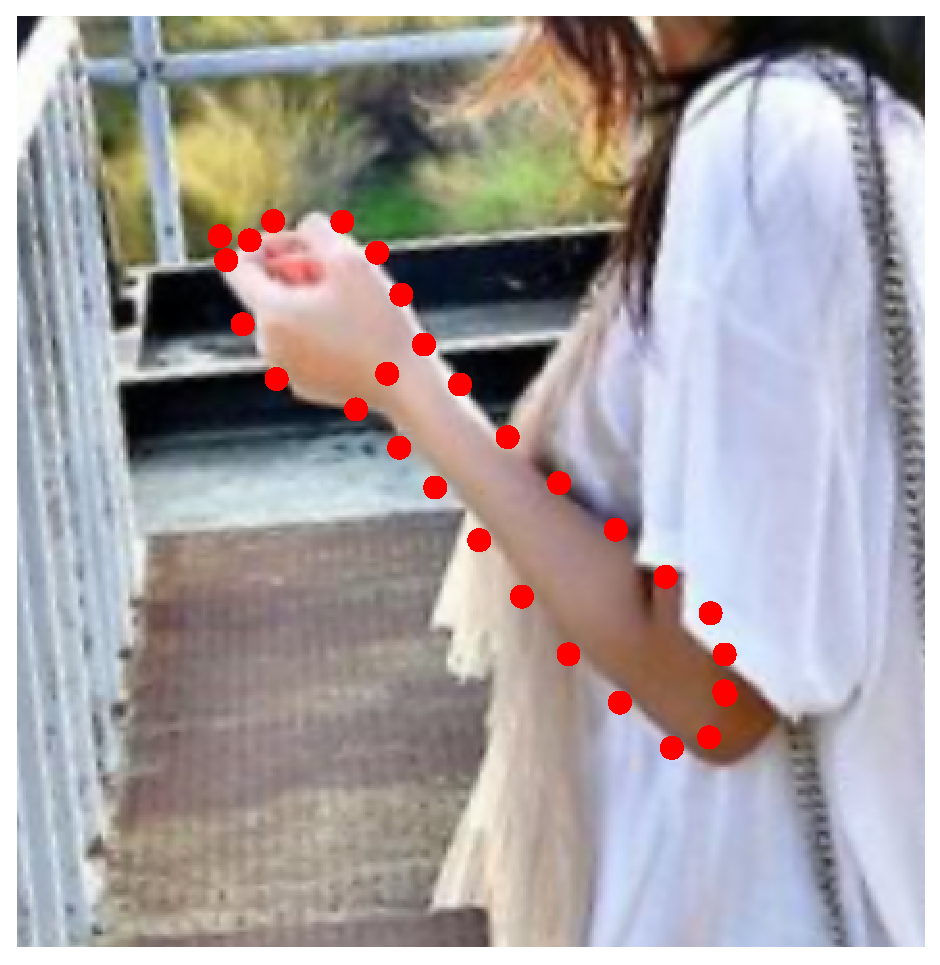
\includegraphics[height=\ofh]{resources/Fittings/25.eps}
    \hfill
    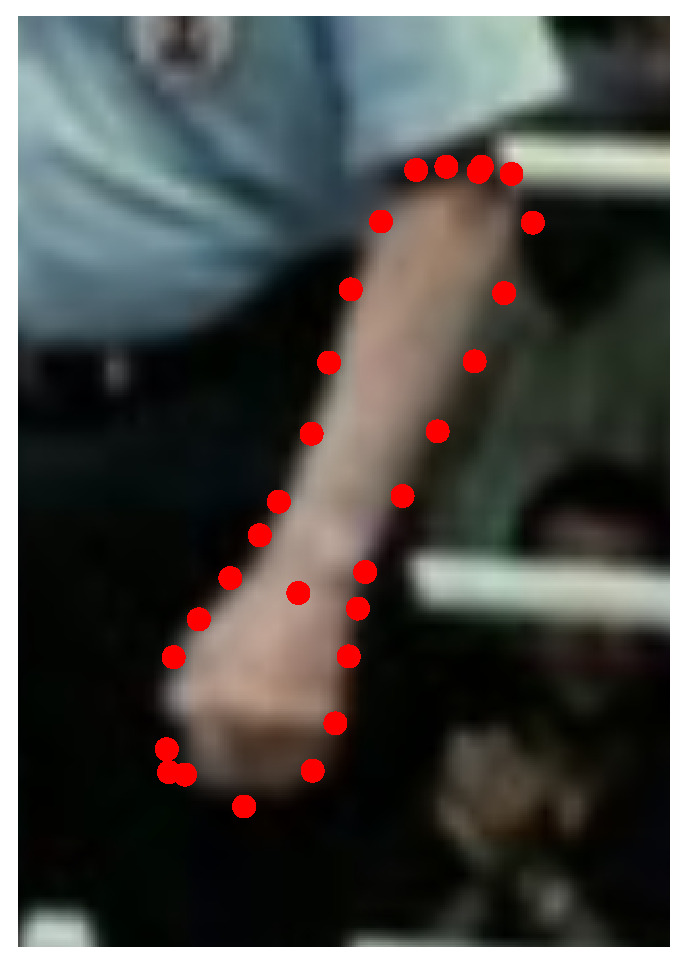
\includegraphics[height=\ofh]{resources/Fittings/27.eps}
    \hfill
    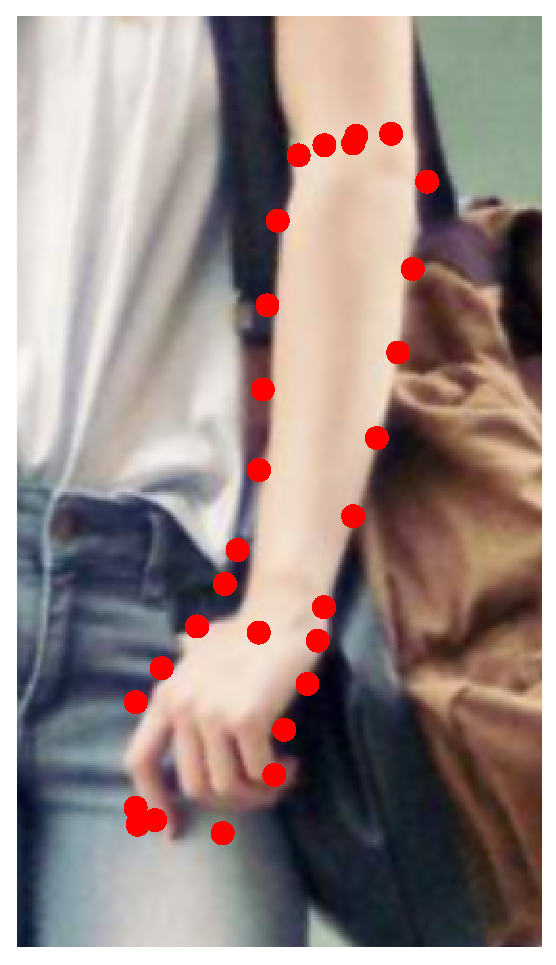
\includegraphics[height=\ofh]{resources/Fittings/29.eps}
    \hfill
    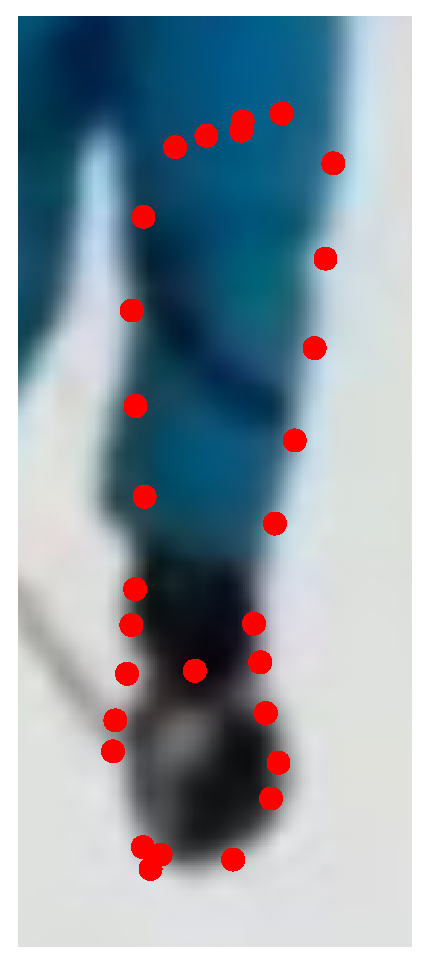
\includegraphics[height=\ofh]{resources/Fittings/31.eps}
    \hfill
    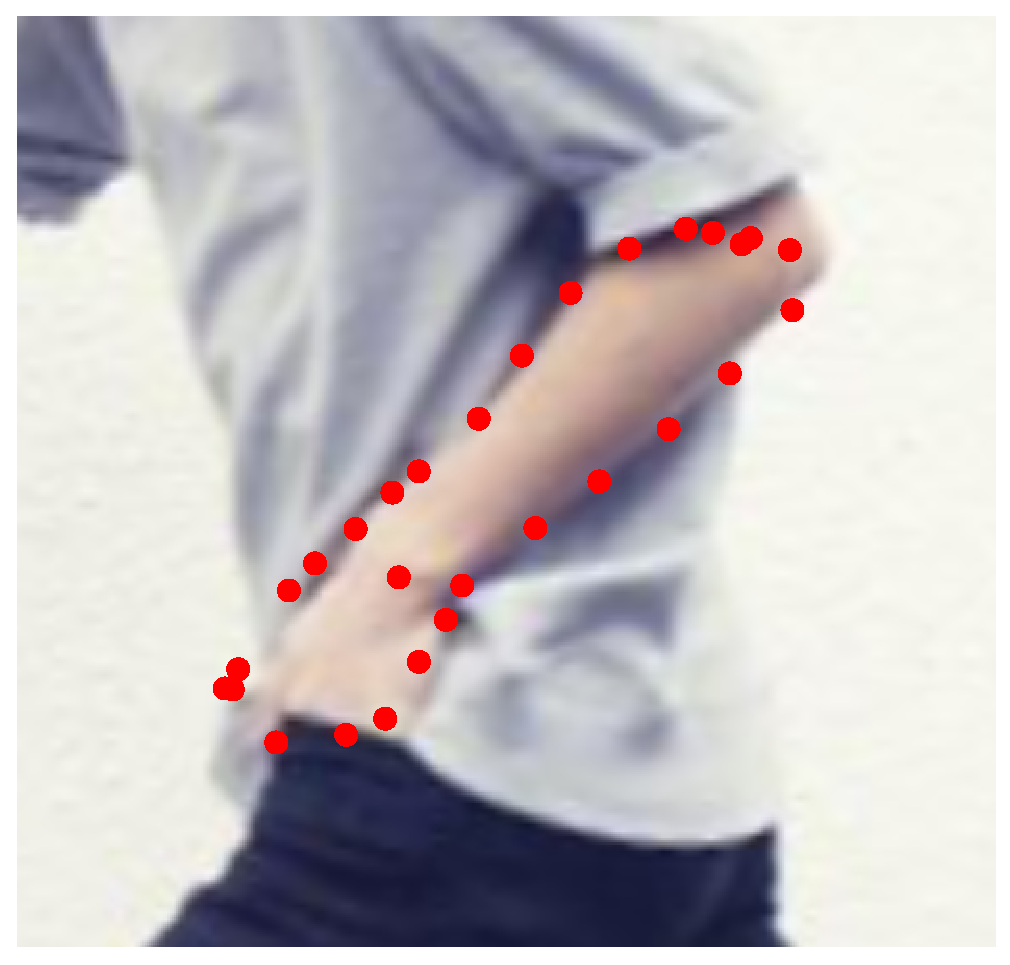
\includegraphics[height=\ofh]{resources/Fittings/33.eps}
    \hfill
    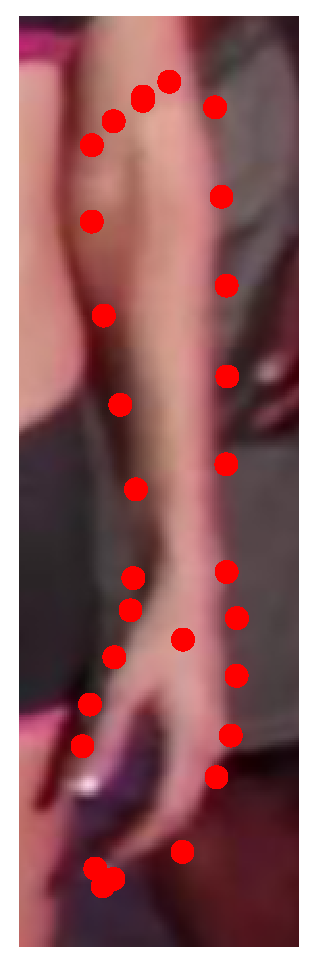
\includegraphics[height=\ofh]{resources/Fittings/35.eps}
    \hfill
    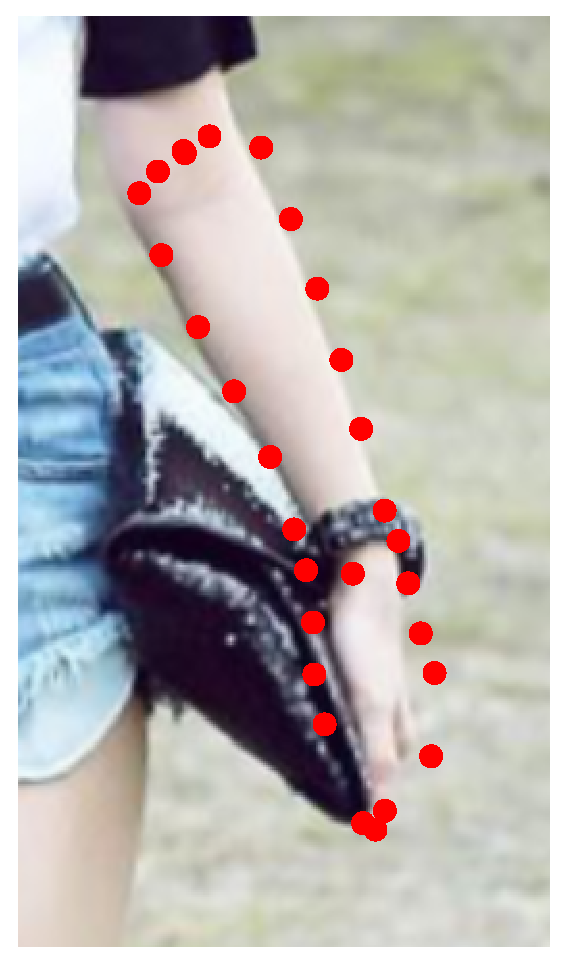
\includegraphics[height=\ofh]{resources/Fittings/36.eps}
    \hfill
    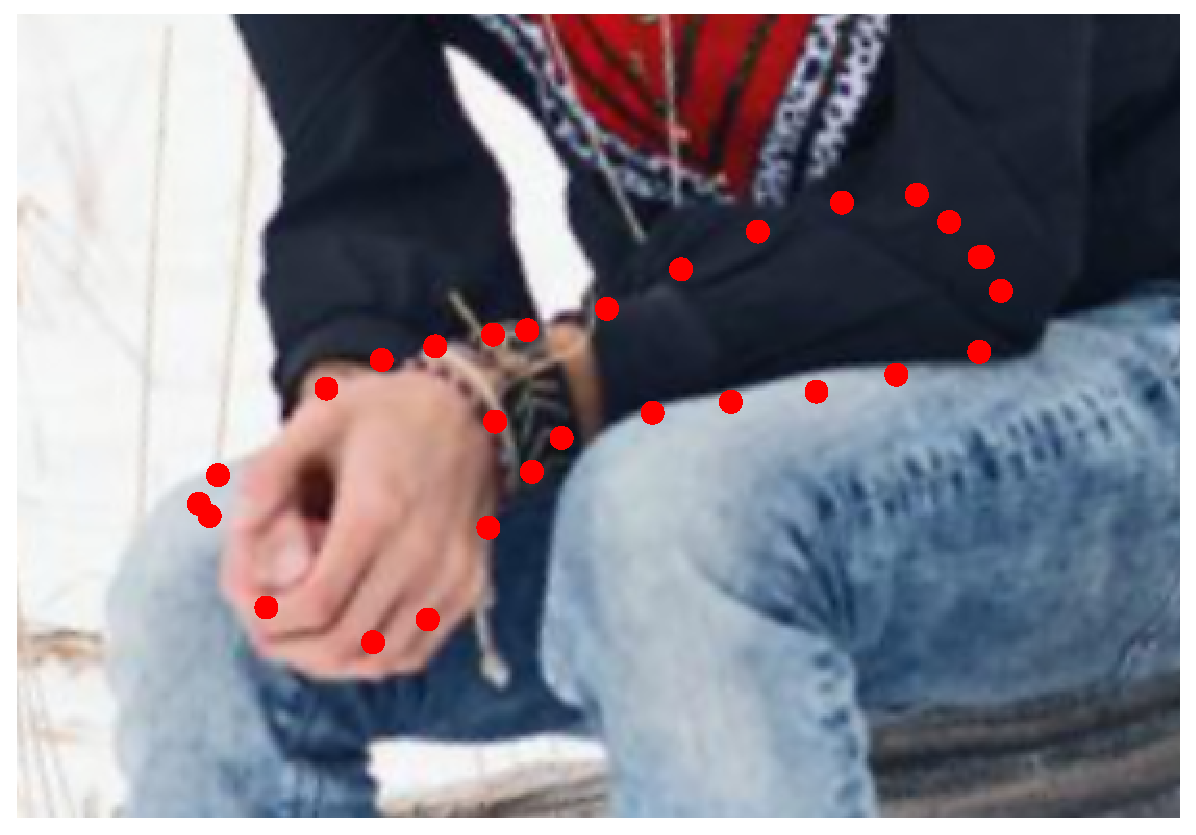
\includegraphics[height=\ofh]{resources/Fittings/37.eps}
    \hfill
    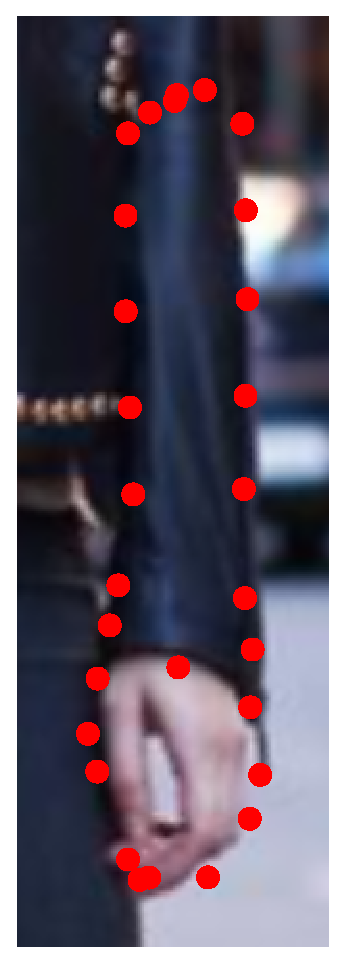
\includegraphics[height=\ofh]{resources/Fittings/38.eps}
    \hfill
    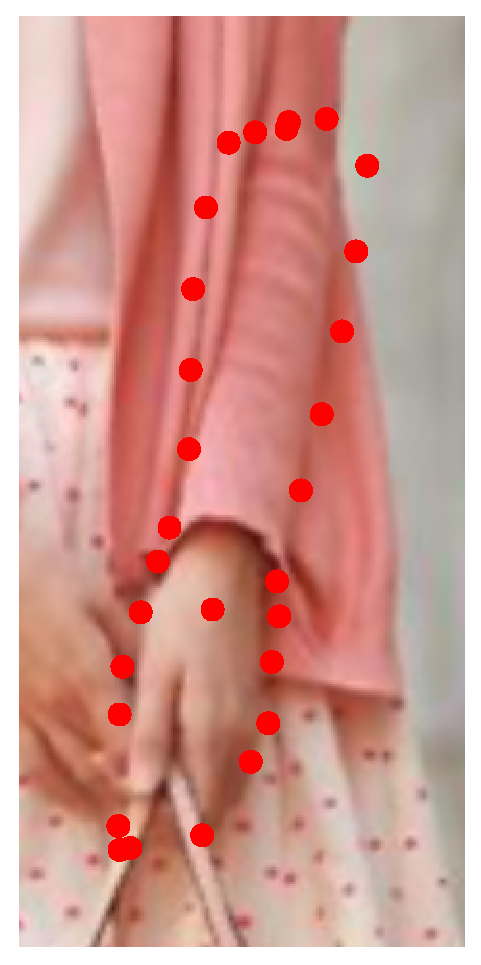
\includegraphics[height=\ofh]{resources/Fittings/39.eps}
    \caption{Demonstration of outline fitting of patch-based AAM on arms.}
    \label{fig:outline_fitting}
    \vspace{-5pt}
\end{figure*}




\subsection{Non-rigid Object Alignment In-the-Wild}
\label{exp:daam_benchmark}
Herein, we compare the fitting accuracy of the dAAMs that are trained with our proposed framework with holistic sparse AAMs~\cite{Cootes2001,Matthews2004,antonakos2015feature}. We consider two object classes that demonstrate rich texture: face and ear.

\noindent\textbf{Databases \& Error Metrics} In the case of face, we trained both models using the 811 training images of the Labelled Faces Parts in-the-Wild (LFPW)~\cite{belhumeur2013localizing}. Sparse AAMs were built from the 68 points annotations provided by~\cite{sagonas_iccv_300w_2013,sagonas2016faces}. Our dAAMs were built as described in Step~\ref{sec:step4}. In both cases, the appearance is represented using pixel intensities. The results are reported on the 224 images of the LFPW testset. The fitting error is evaluated as the point-to-point distance normalised by the face's size, as proposed in~\cite{Zhu2012}.

In the case of human ear, given the lack of publicly available annotated databases, we collected 605 high resolution images captured under unconstrained conditions from online search engines. The images were manually annotated with respect to 55 sparse landmarks, as well as the curve annotations proposed in this paper. Examples of these two types of annotations are shown in Figure~\ref{fig:intro}. We randomly split the database into two disjoint sets of training (500) and testing (105) images. The training and evaluation of the two models is done in the same way as in the case of face.

\begin{figure}[b!]
    \vspace{-5pt}
    \centering
    \includegraphics[width=0.6\columnwidth]{resources/DAAMBenchmark/legend}
    \\
    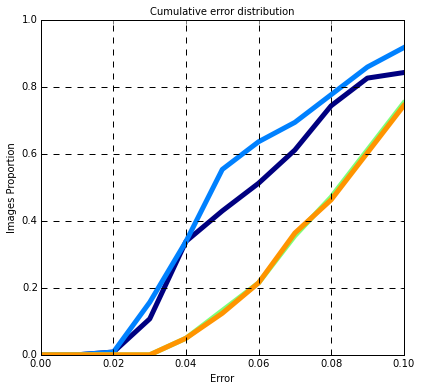
\includegraphics[width=0.48\columnwidth]{resources/DAAMBenchmark/face}
    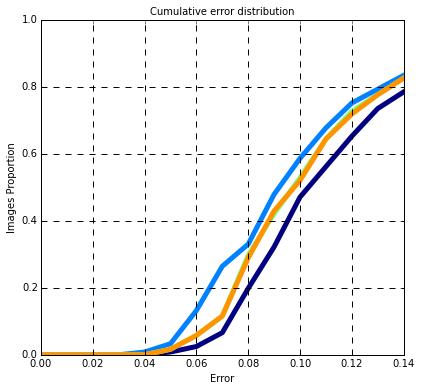
\includegraphics[width=0.48\columnwidth]{resources/DAAMBenchmark/ear}
    \caption{CEDs of faces and ears fitting performance for the experiment of Section \ref{exp:daam_benchmark}.}
    \label{fig:daam_benchmark}
\end{figure}

\noindent\textbf{Results} We report the results in Figure~\ref{fig:daam_benchmark} using Cumulative Error Distribution (CED) curves. By visual inspection of the results, we determined that the fitting is adequately accurate for errors less than 0.1 and 0.06 for the ear and face, respectively. The results indicate that dAAMs marginally outperform sparse AAMs. Therefore, the proposed pipeline is capable of dealing with the complex structure of non-rigid shapes and train dAAMs from simple curve line annotations which can compete and even outperform the commonly-used sparse AAMs trained on carefully annotated images.


\subsection{Arm Pose Estimation}
\label{exp:benchmark}
In this experiment, we aim to compare the effect of training a deformable model of human arm using: (i)~our proposed outline sparse landmarks, and (ii)~the standard skeleton joints annotations that are commonly employed in literature. For this purpose, we employ the patch-based AAM as described in Step~\ref{sec:step4}. Additionally, we compare our methodology with the current state-of-the-art.


\begin{figure}[b!]
    \vspace{-5pt}
    \centering
    \includegraphics[width=\columnwidth]{resources/HandBenchmark/legend}
    \\
    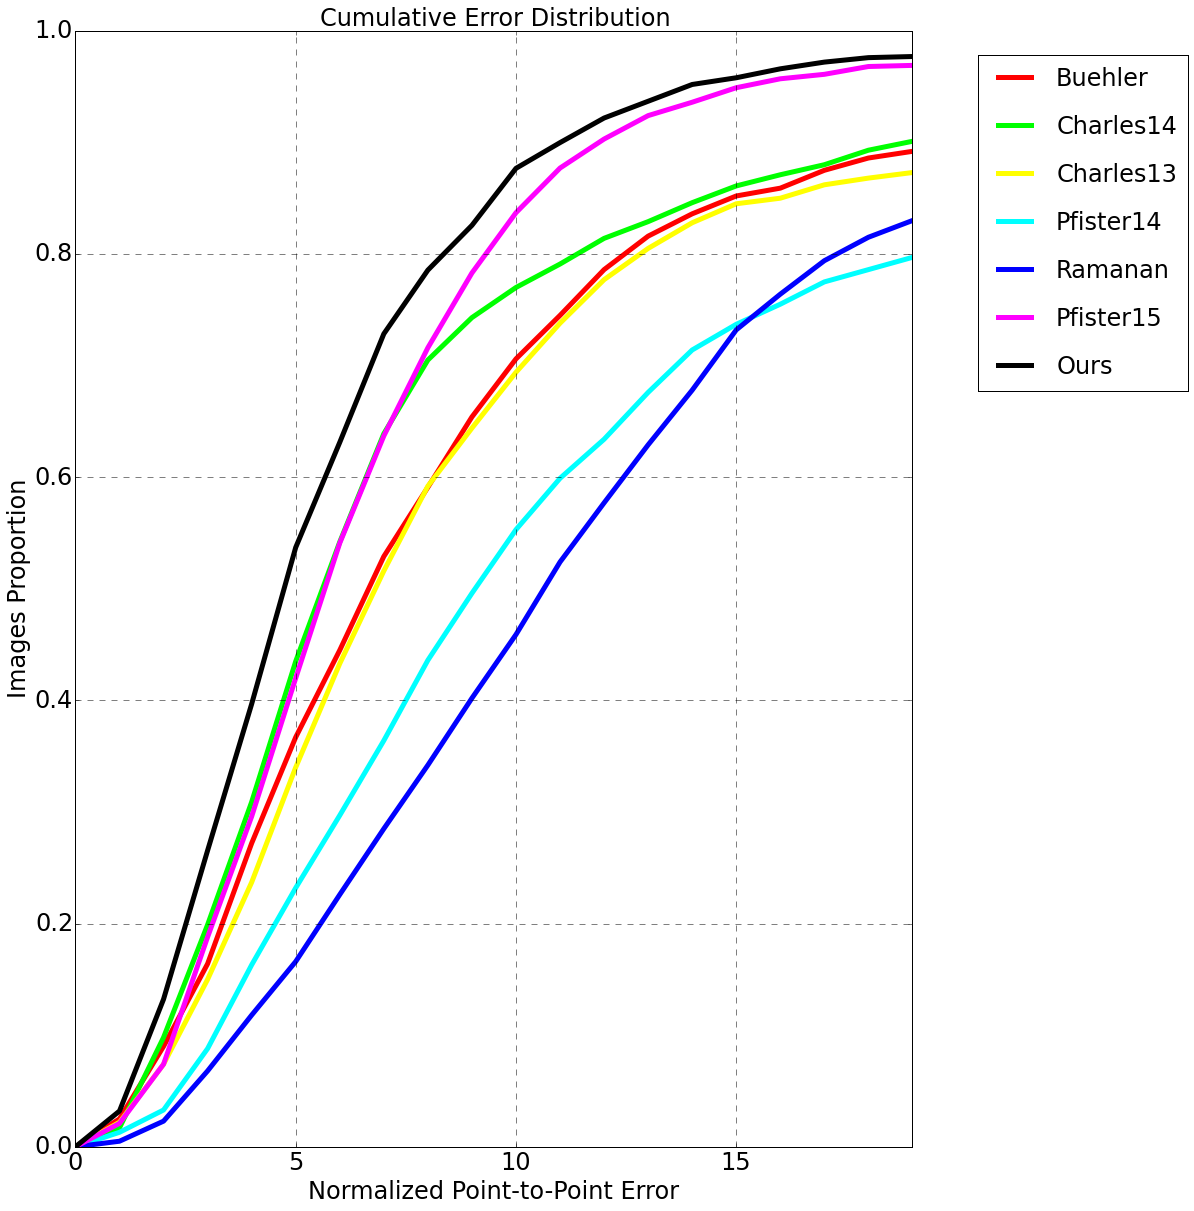
\includegraphics[width=0.48\columnwidth]{resources/HandBenchmark/wrist}
    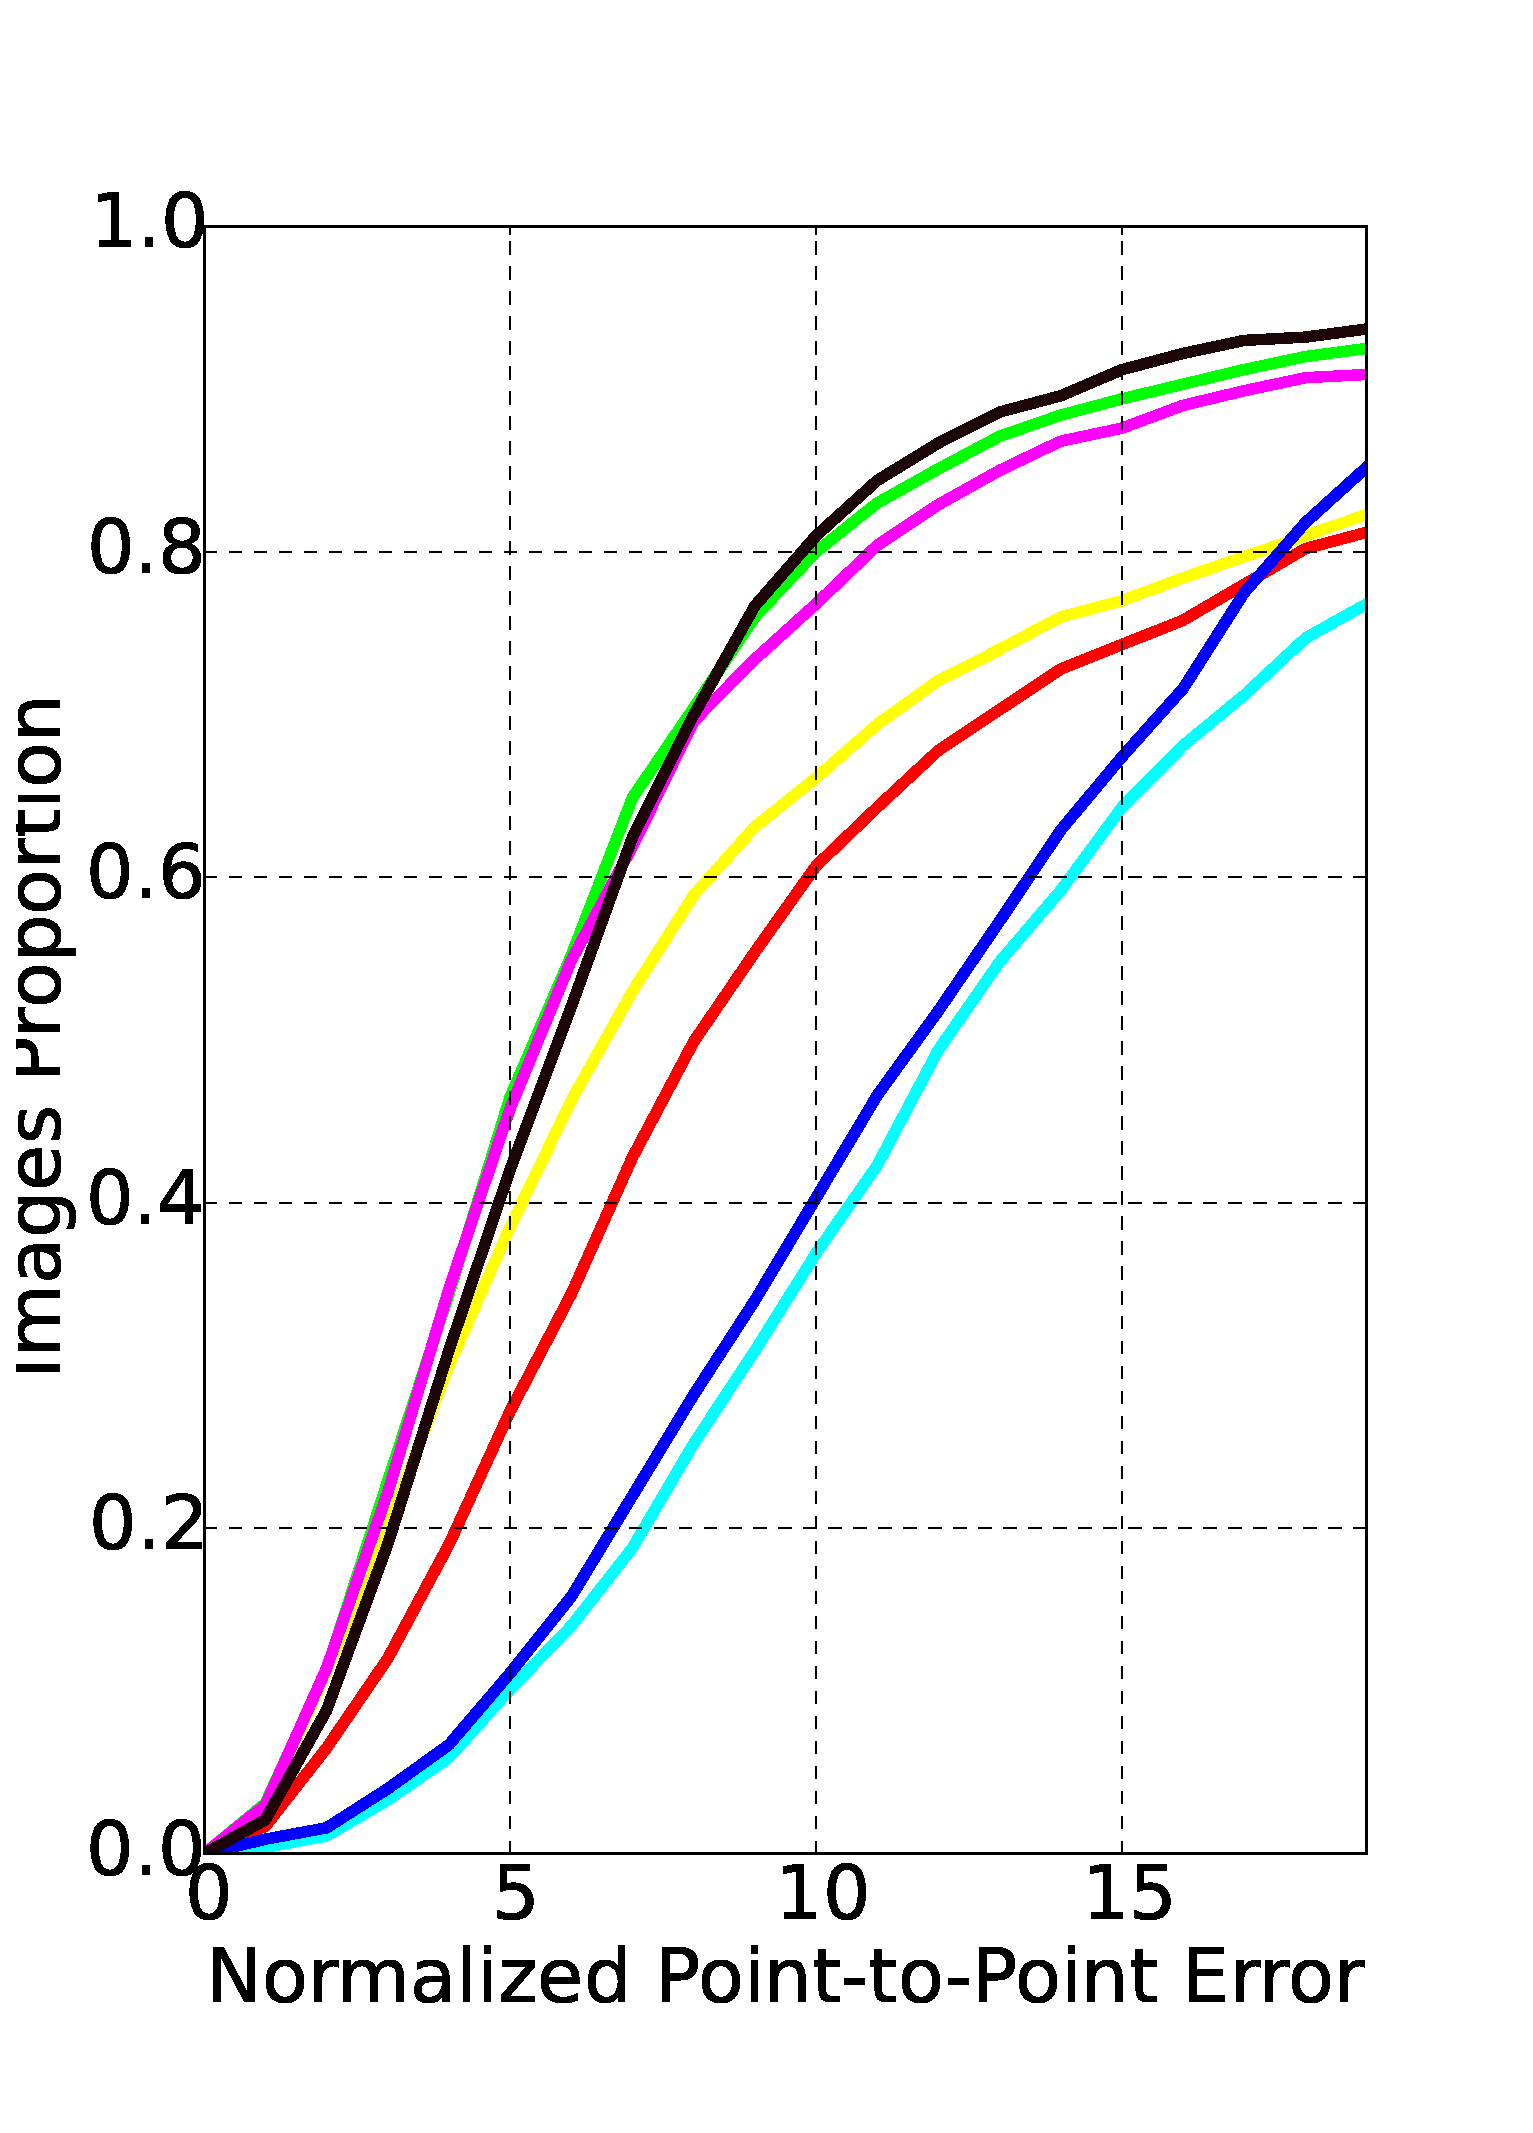
\includegraphics[width=0.48\columnwidth]{resources/HandBenchmark/elbow}
    \caption{CEDs over skeleton landmarks on BBC Pose database for the experiment of Section  \ref{exp:benchmark}.}
    \label{fig:hand_benchmark}
\end{figure}


\noindent\textbf{Dataset \& Error Metric} We opted to report quantitative results on the BBC Pose database~\cite{pfister2015flowing}, which provides the most consistent and accurate joints annotations compared to the rest of existing databases. The training of the outline patch-based AAM was performed after obtaining 29 outline landmarks using our proposed framework. We used 891 training images from a combination of datasets, including H3D~\cite{PoseletsICCV09}, Microsoft COCO~\cite{lin2014microsoft}, MPII~\cite{andriluka14cvpr}, Fashion Pose~\cite{dantone2013human}, FLIC~\cite{sapp2013modec} and BBC Pose~\cite{pfister2015flowing}. SIFT features~\cite{PoseletsICCV09} are adopted for the image representation in our model. The fitting procedure on the BBC Pose database is initialised using a simplistic in-house deep convolutional neural network.

In order to compare with current state-of-the-art on BBC Pose, we used the same error metric as the one in~\cite{pfister2015flowing}, which normalises testing images in order to have a height of 256 pixels. Once again, the performance is visualised using CED curves. The results for this experiment are reported on 1000 testing images from BBC Pose, which utilises 7 skeleton landmarks to annotate the human upper-body pose. Note that in the case of our model, the final joints locations required for evaluation are retrieved from the dense correspondence acquired with our proposed method. On the contrary, the rest of the methods are trained on this 7-points mark-up, thus directly return their estimated locations.

\noindent\textbf{Results} Figure~\ref{fig:hand_benchmark} reports the results of our model trained on the outline landmarks (Outline PAAM), as well as the current state-of-the-art techniques which include: Buehler~\cite{buehler2011upper}, Charles14~\cite{charles2014upper}, Charles13~\cite{charles2013domain}, Pfister14~\cite{pfister2015deep}, Ramanan~\cite{yang2013articulated} and Pfister15~\cite{pfister2015flowing}. As can be seen, our outline part-based AAM model outperforms the state-of-the-art for this task, even though it is not trained directly on the wrist and elbow points, thus it is not tailored for locating them. In particular, our model outperforms the currently best method~\cite{pfister2015flowing} by a notable amount (9\% with error less than 6pt) on wrist, as well as marginal improvement on elbow estimation. Figure~\ref{fig:outline_fitting} shows some indicative qualitative fitting results.

In the same experiment we prove that it is more advantageous to train a deformable model using the outline landmarks rather than the skeleton points. This is done by building a patch-based AAM on the same training data and with identical settings using both annotation schemes. As it can be seen from the  CED curves of Figure~\ref{fig:hand_benchmark}, our model trained on outline landmarks (Outline PAAM) notable outperforms the skeleton-based model for both wrist and elbow. We believe that this is a remarkable result, which indicates that out proposed outline mark-up can lead to a significant improvement of current state-of-the-art techniques.


% \begin{figure*}[!t]
%     \newcommand{\fh}{0.24\columnwidth}
%     \centering
%     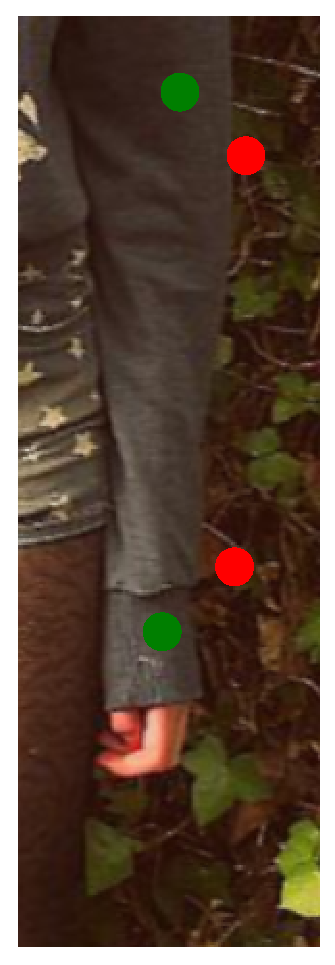
\includegraphics[height=\fh]{resources/Fixing/fix_1}
%     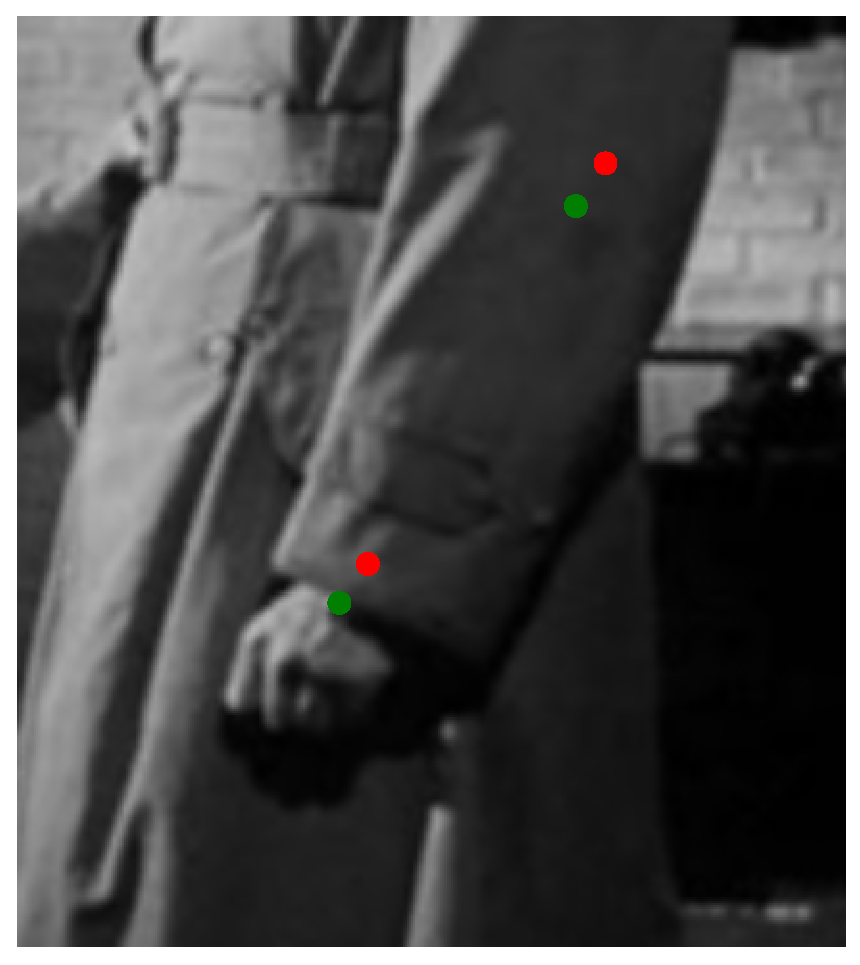
\includegraphics[height=\fh]{resources/Fixing/fix_2}
%     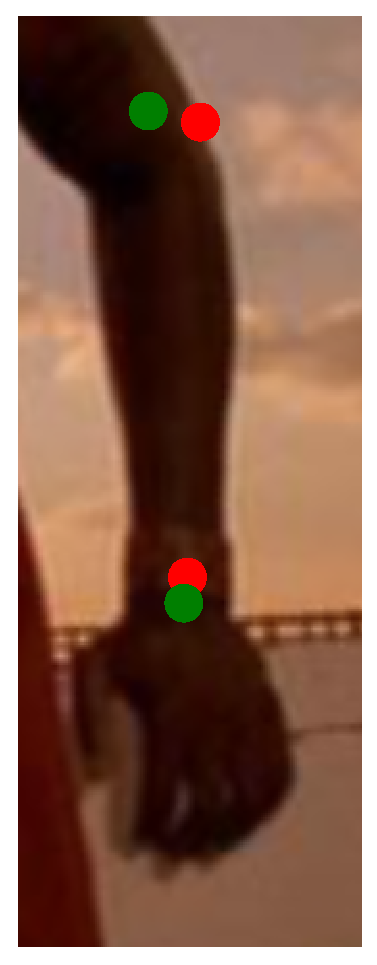
\includegraphics[height=\fh]{resources/Fixing/fix_3}
%     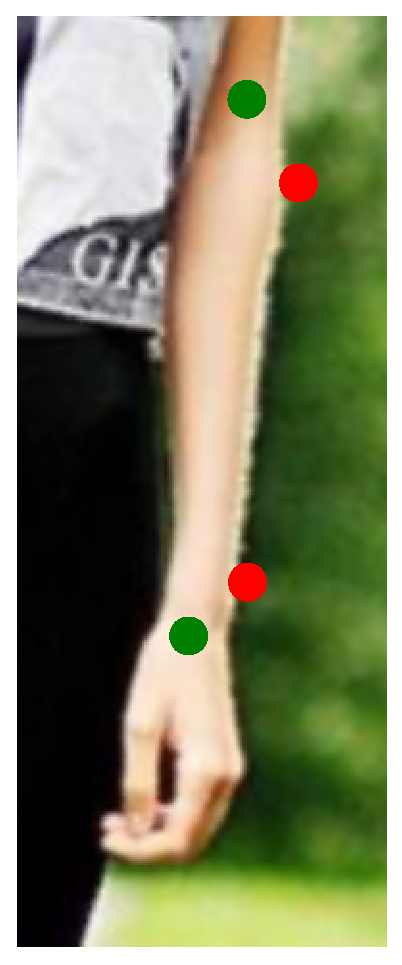
\includegraphics[height=\fh]{resources/Fixing/fix_5}
%     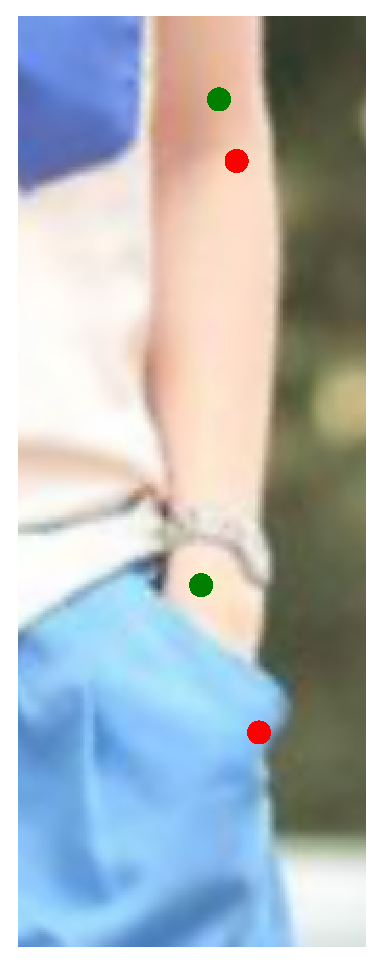
\includegraphics[height=\fh]{resources/Fixing/fix_6}
%     \includegraphics[height=\fh]{resources/Fixing/fix_7}
%     \includegraphics[height=\fh]{resources/Fixing/fix_8}
%     \includegraphics[height=\fh]{resources/Fixing/fix_9}
%     \includegraphics[height=\fh]{resources/Fixing/fix_10}
%     \includegraphics[height=\fh]{resources/Fixing/fix_20}
%     \includegraphics[height=\fh]{resources/Fixing/fix_12}
%     \includegraphics[height=\fh]{resources/Fixing/fix_13}
%     \includegraphics[height=\fh]{resources/Fixing/fix_14}
%     \includegraphics[height=\fh]{resources/Fixing/fix_15}
%     \includegraphics[height=\fh]{resources/Fixing/fix_17}
%     \includegraphics[height=\fh]{resources/Fixing/fix_18}
%     \caption{Demonstration of annotation correction using our method for experiment \ref{exp:qualitative}. \emph{Red} dots refer to officially provided landmarks, and \emph{green} dots are corrected position.}
%     \label{fig:qualitative}
% \end{figure*}

% \begin{figure*}[!t]
%     \newcommand{\ofh}{0.24\columnwidth}
%     \centering
%     \includegraphics[height=\ofh]{resources/Fittings/20.eps}
%     \includegraphics[height=\ofh]{resources/Fittings/3.eps}
%     \includegraphics[height=\ofh]{resources/Fittings/19.eps}
%     \includegraphics[height=\ofh]{resources/Fittings/4.eps}
%     \includegraphics[height=\ofh]{resources/Fittings/6.eps}
%     \includegraphics[height=\ofh]{resources/Fittings/15.eps}
%     \includegraphics[height=\ofh]{resources/Fittings/7.eps}
%     \includegraphics[height=\ofh]{resources/Fittings/8.eps}
%     \includegraphics[height=\ofh]{resources/Fittings/13.eps}
%     \includegraphics[height=\ofh]{resources/Fittings/17.eps}
%     \\
%     \includegraphics[height=\ofh]{resources/Fittings/21.eps}
%     \includegraphics[height=\ofh]{resources/Fittings/23.eps}
%     \includegraphics[height=\ofh]{resources/Fittings/25.eps}
%     \includegraphics[height=\ofh]{resources/Fittings/27.eps}
%     \includegraphics[height=\ofh]{resources/Fittings/29.eps}
%     \includegraphics[height=\ofh]{resources/Fittings/31.eps}
%     \includegraphics[height=\ofh]{resources/Fittings/33.eps}
%     \includegraphics[height=\ofh]{resources/Fittings/35.eps}
%     \includegraphics[height=\ofh]{resources/Fittings/36.eps}
%     \includegraphics[height=\ofh]{resources/Fittings/37.eps}
%     \includegraphics[height=\ofh]{resources/Fittings/38.eps}
%     \includegraphics[height=\ofh]{resources/Fittings/39.eps}
%     \caption{Demonstration of outline fitting of patch-based AAM on arms.}
%     \label{fig:outline_fitting}
% \end{figure*}

\subsection{Annotation Correction}
\label{exp:qualitative}
The final experiment demonstrates that it is feasible to use the proposed arm model in order to correct the annotations provided by current datasets. As mentioned above there are inconsistencies in the annotations of MPII~\cite{andriluka14cvpr}, Fashion Pose~\cite{dantone2013human} and FLIC~\cite{sapp2013modec}. Due to the large variance in arm pose, it is difficult even for trained annotators to obtain consistent annotations between them. As proof of concept, Figure~\ref{fig:variance} reports the standard deviation observed between the annotations of 4 trained humans that were requested to annotate 120 images of left arms from Fashion Pose~\cite{dantone2013human} with respect to the shoulder, elbow and wrist.

By applying our outline patch-based AAM on the aforementioned databases, we managed to greatly correct the currently available annotations of the arm. Figure~\ref{fig:qualitative} shows indicative examples of the corrected landmarks. There is no doubt that points after correction demonstrate more consistency among images. We make the corrected annotations publicly available\textsuperscript{\ref{foot:annotations}}.


















% \begin{table}[b!]
%     \small
%     \centering
%     \begin{tabular}{|l|c|c|c||c|c|c|}
%         \hline
%                             & \multicolumn{3}{c||}{Wrist} & \multicolumn{3}{c|}{Elbow}\\
%         \hline
%         \emph{Method}       & \emph{mean} & \emph{std} & $\leq 6pt$ & \emph{mean} & \emph{std} & $\leq 6pt$\\
%         \hline\hline
%         Buehler             & 12.08    & 19.94        & 44.5\%       & 12.94    & 14.65        & 34.4\%\\
%         Charles14           & 11.81    & 20.89        & 54.2\%       &  8.30    & 11.00        & \textbf{55.2\%}\\
%         Charles13           & 13.78    & 22.39        & 43.3\%       & 13.17    & 18.74        & 46.3\%\\
%         Pfister14           & 14.69    & 17.89        & 29.7\%       & 14.60    & 10.59        & 14.0\%\\
%         Ramanan             & 15.59    & 19.04        & 22.6\%       & 15.53    & 10.82        & 15.8\%\\
%         Pfister15           & 7.62     & 11.04        & 54.1\%       &  8.84    & 11.44        & 54.9\%\\
%         \hline\hline
%         Ours                & \textbf{6.71}& \textbf{10.90}   & \textbf{63.1\%}       & \textbf{8.20}     &  \textbf{10.54}        & 52.1\%\\
%         \hline
%     \end{tabular}
%     \caption{Fitting statistics on BBC Pose database for experiment \ref{exp:benchmark}}
%     \label{tab:hand_benchmark}
